\documentclass[11pt,a4paper]{article}
\usepackage[utf8]{inputenc}
\usepackage[english]{babel}
\usepackage{geometry}
\geometry{margin=1in}
\usepackage{graphicx}
\usepackage{hyperref}
\usepackage{minted}
\usepackage{titlesec}
\usepackage{fancyhdr}
\usepackage{caption}
\usepackage{enumitem}
\usepackage{listings}
\usepackage{xcolor}
\usepackage{float}
\usepackage{amsmath}

% Code highlighting
\lstset{
  basicstyle=\ttfamily\small,
  breaklines=true,
  backgroundcolor=\color{gray!10},
  frame=single,
}
\lstdefinelanguage{yaml}{
  keywords={true,false,null,y,n},
  keywordstyle=\color{blue},
  basicstyle=\ttfamily\small,
  sensitive=false,
  comment=[l]{\#},
  morecomment=[l]{\#},
  commentstyle=\color{gray}\ttfamily,
  morestring=[b]',
  morestring=[b]"
}
\lstdefinelanguage{dart}{
  morekeywords={
    async, await, break, case, catch, class, const, continue, default, do, else, enum, export,
    extends, external, factory, false, final, finally, for, if, implements, import, in, interface,
    is, new, null, on, override, part, rethrow, return, set, static, super, switch, this, throw,
    true, try, typedef, var, void, while, with, yield
  },
  sensitive=true,
  morecomment=[l]{//},
  morecomment=[s]{/*}{*/},
  morestring=[b]",
  morestring=[b]',
  keywordstyle=\color{blue}\bfseries,
  commentstyle=\color{gray}\ttfamily,
  stringstyle=\color{orange},
  basicstyle=\ttfamily\small,
}

\lstdefinelanguage{json}{
  morestring=[b]",
  morecomment=[l]{//},
  moredelim=**[is][\color{blue}]{@}{@},
  stringstyle=\color{orange},
  commentstyle=\color{gray},
  basicstyle=\ttfamily\small,
}

% Header and footer
\pagestyle{fancy}
\fancyhf{}
\rhead{Project Documentation}
\lhead{Rocket App}
\rfoot{\thepage}

% Section formatting
\titleformat{\section}{\normalfont\Large\bfseries}{\thesection}{1em}{}
\titleformat{\subsection}{\normalfont\large\bfseries}{\thesubsection}{1em}{}

% Custom commands
\newcommand{\email}[1]{\texttt{#1}}
\newcommand{\id}[1]{\texttt{#1}}

% Title page
\begin{document}

\begin{titlepage}
    \begin{flushright}
        
\includegraphics[width=4cm]{images/Logo-HFT-Stuttgart.png}
    \end{flushright}
    \vspace{0.5cm}

    \begin{center}
        {\Huge \textbf{Rocket App} \par}
        \vspace{0.3cm}
        {\LARGE \textit{Pervasive Computing} \par}
        \vspace{1.5cm}
        
\includegraphics[width=5cm]{images/AppIcon.png}
        \vspace{1.5cm}

        {\Large Autoren: \par}
        \vspace{0.3cm}
        \begin{tabular}{rl}
            Paul Durz      & \email{22dupa1bif@hft-stuttgart.de} \\
                          & Matrikelnummer: \id{1005080} \\
            Dominik Gräter & \email{22grdo1bif@hft-stuttgart.de} \\
                          & Matrikelnummer: \id{1005093} \\
            Manuel Holm    & \email{22homa1bif@hft-stuttgart.de} \\
                          & Matrikelnummer: \id{1005094} \\
            Ron Seifried   & \email{22sero1bif@hft-stuttgart.de} \\
                          & Matrikelnummer: \id{1005466} \\
        \end{tabular}
        \vspace{1.5cm}

        \textbf{Hochschule für Technik Stuttgart} \\
        Schellingstraße 24, 70174 Stuttgart, Deutschland \\
        \email{info@hft-stuttgart.de} \\
        \url{https://www.hft-stuttgart.de/}

        \vfill
        \large Abgabedatum: \today \\
    \end{center}
\end{titlepage}

\tableofcontents

\newpage
\addcontentsline{toc}{section}{Abbildungsverzeichnis}
\listoffigures
\newpage

\section{Einleitung}
Im Rahmen des Moduls Ubiquitous Computing von Professor Knauth sollten die
Studierenden das Erlernte in einem praktischen Projekt anwenden.
Das Projekt beschäftigt sich mit der Thematik des Ubiquitous Computings. Die
Durchdringung von Alltagsgegenständen mit Informationstechnologie und die
Vernetzung von smarten Systemen führen zu einer Umwelt, in der in allen Bereichen
Veränderungen auftreten. Wir haben uns dabei für eine Mobile App für Smartphones entschieden.

\subsection{Projektbeschreibung}
Die \textbf{Rocket App} ist eine mobile Anwendung, die es Nutzerinnen und Nutzern ermöglicht, ihre täglichen Schritte automatisch zu erfassen. Die App belohnt Aktivität durch ein Punktesystem, das sowohl auf der Anzahl der Schritte als auch auf der Teilnahme an Herausforderungen (Challenges) basiert. Zusätzlich können Läufe (Runs) aufgezeichnet, auf Karten dargestellt und im Nachhinein analysiert werden. Die Kombination aus Bewegungstracking, Gamification und sozialem Vergleich macht die Rocket App zu einem motivierenden Begleiter im Alltag.

\subsection{Ziele und Motivation}
Ziel der Rocket App ist es, Nutzerinnen und Nutzer zu einem aktiveren Lebensstil zu motivieren. Durch spielerische Elemente wie Punkte, Ranglisten und Challenges soll Bewegung im Alltag gefördert und langfristig zur Gewohnheit gemacht werden. Gerade im Kontext zunehmender Digitalisierung und Bewegungsmangel bietet die App eine niedrigschwellige Möglichkeit, körperliche Aktivität zu fördern und messbar zu machen.

\subsection{Website}
Für die Möglichkeit, die App mit einer Website erweitern zu dürfen, danken wir Professor Dr. Knauth und Prof. Dr. Mosler.
Diese Erweiterungen und die Darstellung der App auf einer Website sind nicht Teil der Pervasive Computing Vorlesung, gehören aber zu unserem Projekt dazu und sollten hier nicht unerwähnt bleiben.

Die Website bietet dieselben Features wie die App, man kann aber auch noch Runs planen, man hat einen globalen Chat und man hat die Möglichkeit, die App zu downloaden.
Die Website ist über diesen Link einsehbar \url{https://rocket-app.social}.

Die Zielgruppe der App sind Menschen, die ihre Bewegung im Alltag tracken und sich selbst oder im Wettbewerb mit anderen motivieren möchten. Dazu gehören sowohl Gelegenheitsnutzer als auch sportlich Aktive.

\section{Entwicklung}
\subsection{Versionsverwaltung}
Für die Entwicklung der \textbf{Rocket App} wurde ein zentrales Git-Repository unter GitHub verwendet. Im Zuge dessen haben wir eine eigene Organisation namens \texttt{RealTeamRocket} auf GitHub gegründet, um die Projektressourcen zentral zu verwalten und die Zusammenarbeit im Team zu erleichtern. Das Repository ist unter folgendem Link öffentlich einsehbar:
\url{https://github.com/RealTeamRocket/rocket-app}

Das Repository enthält sämtliche Quellcodes des Projekts – darunter das Flutter-Frontend der App, das Backend sowie eine begleitende Website. Durch diese zentrale Struktur wird sichergestellt, dass alle Komponenten konsistent versioniert und gepflegt werden können.

Zur effizienten Zusammenarbeit im Team wurde mit einem \textbf{Branching-Modell} gearbeitet. Dabei existieren Hauptzweige wie \texttt{main} und \texttt{dev}, während neue Features oder Bugfixes in separaten Feature-Branches entwickelt und anschließend via Pull Request integriert wurden. Dieses Vorgehen erlaubt paralleles Arbeiten, minimiert Merge-Konflikte und sorgt für eine saubere Trennung zwischen stabilen Releases und laufender Entwicklung.

Zur Sprint-Planung und Aufgabenverteilung kommt zusätzlich ein \textbf{GitHub Project Board} zum Einsatz, das als Kanban-Board konfiguriert wurde. Dort werden Tickets angelegt, priorisiert und den jeweiligen Teammitgliedern zugewiesen. Das Board dient als zentrale Planungsgrundlage für unsere zweiwöchigen Sprints und bietet eine transparente Übersicht über den Fortschritt einzelner Aufgaben und Meilensteine.

Durch die Kombination aus GitHub, strukturiertem Branch-Workflow und projektbezogener Aufgabenplanung konnte eine effektive und nachvollziehbare Versionskontrolle realisiert werden, die sowohl technische als auch organisatorische Anforderungen erfüllt.

\subsection{Entwicklungsumgebungen}

Für die Entwicklung der \textbf{Rocket App} kamen unterschiedliche Entwicklungsumgebungen zum Einsatz, abgestimmt auf die jeweiligen Anforderungen der Frontend- und Backend-Komponenten.

Die App wurde mit dem Framework \textbf{Flutter}\cite{flutter} entwickelt. Für die mobile Entwicklung wurde hauptsächlich \textbf{Android Studio}\cite{androidstudio} verwendet, insbesondere für das Erstellen, Debuggen und Testen auf realen Geräten sowie Emulatoren. Ergänzend kam auch der integrierte \textbf{Emulator von Visual Studio Code (VS Code)}\cite{VSCode} zum Einsatz, insbesondere für schnelle Tests und kleinere Anpassungen während der Entwicklung. Dank der Flutter-Integration in beide Umgebungen konnten Entwickler flexibel je nach Präferenz arbeiten.

Für das \textbf{Backend}, das in der Programmiersprache \textbf{Go}\cite{golang} entwickelt wurde, war die Wahl der Entwicklungsumgebung weitgehend frei. Da Go standardmäßig nur über den Go Language Server Protocol (gopls)\cite{gopls} unterstützt wird, kamen primär Editoren mit entsprechender LSP-Unterstützung zum Einsatz. Die bevorzugten Tools waren hier \textbf{Visual Studio Code} sowie der moderne Editor \textbf{Zed}\cite{zed}, welcher sich durch seine Performance und klare Nutzeroberfläche auszeichnet. Beide Umgebungen bieten durch die LSP-Anbindung komfortable Features wie Autovervollständigung, Syntaxhervorhebung und Code-Navigation.

Durch diese vielseitige Toolauswahl konnten alle Projektbeteiligten in einer für sie optimalen Umgebung arbeiten, ohne auf zentrale Entwicklungsfeatures verzichten zu müssen. Dies förderte eine produktive Arbeitsweise und erhöhte die Effizienz im Entwicklungsalltag.

\subsection{Virtual Private Server}

Für das Hosting der Server-Komponenten der \textbf{Rocket App} wird ein \textbf{Virtual Private Server (VPS)} von \textbf{Oracle Cloud} genutzt. Auf diesem Server laufen sowohl das \textbf{Backend} als auch die dazugehörige \textbf{PostgreSQL-Datenbank}\cite{postgresql}. Um die Dienste zuverlässig und portabel zu betreiben, werden beide Komponenten in separaten \textbf{Docker-Containern}\cite{docker} ausgeführt.

Die Orchestrierung dieser Container erfolgt über eine \textbf{Docker Compose}-Konfiguration, die das Starten, Stoppen und Verwalten der Services vereinfacht. Zusätzlich kommt das Tool \textbf{Watchtower} zum Einsatz, das regelmäßig nach aktualisierten Docker-Images prüft. Sobald ein neues Image – beispielsweise des Backends – auf \textbf{Docker Hub}\cite{docker_hub} verfügbar ist, lädt Watchtower es automatisch herunter und startet den entsprechenden Container neu. Dadurch wird sichergestellt, dass der Server stets mit der aktuellsten Version läuft, ohne manuelles Eingreifen.

\subsection{Deployment}

Das Deployment des Backends ist vollständig automatisiert und in den Entwicklungsworkflow über \textbf{GitHub-Actions}\cite{github} integriert. Bei jedem \textbf{Pull Request auf den \texttt{master}-Branch}, der Änderungen im Verzeichnis \texttt{rocket-backend} betrifft, wird eine entsprechende GitHub-Action ausgelöst.

Diese Action übernimmt das Erstellen eines neuen Docker-Images auf Basis des aktuellen Codes und lädt es anschließend in ein zentrales \textbf{Docker Hub}-Repository hoch. Sobald das neue Image dort verfügbar ist, erkennt \textbf{Watchtower} auf dem Oracle-Server das Update und sorgt automatisch für einen nahtlosen Rollout der neuen Backend-Version.

Ein Ausschnitt aus dem verwendeten Deployment-Workflow sieht wie folgt aus:

\begin{lstlisting}[language=yaml, caption={GitHub Action zur automatisierten Bereitstellung}, label={lst:deployment}]
name: Build and Push Docker Image

on:
  push:
    branches:
      - master
    paths:
      - 'rocket-backend/**'

jobs:
  build-and-push:
    runs-on: ubuntu-latest

    steps:
      - name: Checkout code
        uses: actions/checkout@v3

      - name: Log in to Docker Hub
        uses: docker/login-action@v2
        with:
          username: ${{ secrets.DOCKER_USERNAME }}
          password: ${{ secrets.DOCKER_PAT }}

      - name: Set up Docker Buildx
        uses: docker/setup-buildx-action@v2

      - name: Build and Push Docker Image
        uses: docker/build-push-action@v4
        with:
          context: ./rocket-backend
          push: true
          tags: ${{ secrets.DOCKER_USERNAME }}/rocket-backend:latest
\end{lstlisting}

Durch diese Pipeline wird das Deployment effizient, reproduzierbar und sicher gestaltet – ein entscheidender Vorteil bei der iterativen Weiterentwicklung der Rocket App.

\subsection{Setup und Lokale Ausführung}
Um das System lokal vollständig auszuführen, werden folgende Tools benötigt:

\begin{itemize}
    \item \textbf{Flutter} -- zum Kompilieren und Starten der mobilen Anwendung
    \item \textbf{Docker \& Docker Compose} -- für das Starten des Backends und der PostgreSQL-Datenbank
\end{itemize}

\subsubsection{1. Backend und Datenbank starten}

Zunächst muss das Backend gemeinsam mit der Datenbank gestartet werden. Dazu navigiert man ins Verzeichnis \texttt{rocket-backend} und führt dort den folgenden Befehl aus:

\begin{verbatim}
docker-compose up --build
\end{verbatim}

Dieser Befehl setzt voraus, dass im selben Verzeichnis eine \texttt{.env}-Datei vorhanden ist. Diese Datei enthält alle Konfigurationsvariablen für Backend und Datenbank. Ein Beispiel-Template sieht wie folgt aus:

\begin{verbatim}
PORT=8080
APP_ENV=local
BLUEPRINT_DB_HOST=postgres
BLUEPRINT_DB_PORT=5432
BLUEPRINT_DB_DATABASE=blueprint
BLUEPRINT_DB_USERNAME=melkey
BLUEPRINT_DB_PASSWORD=password1234
BLUEPRINT_DB_SCHEMA=public

# generated with openssl rand -base64 64
JWT_SECRET=
API_KEY=

PGADMIN_DEFAULT_EMAIL=admin@admin.com
PGADMIN_DEFAULT_PASSWORD=admin
\end{verbatim}

Nach dem Start des Containers wird die Datenbank automatisch durch ein spezielles Migration-Image \texttt{migrate/migrate}\cite{migrate} mit den benötigten Tabellen und Constraints versorgt.

\subsubsection{2. Lokale Kommunikation mit dem Handy aktivieren}

Damit die mobile App während der lokalen Entwicklung mit dem Backend kommunizieren kann, ist es entscheidend, dass das Handy im selben Netzwerk wie der Entwicklungsrechner ist. Zudem muss entweder:

\begin{itemize}
    \item die lokale Firewall deaktiviert oder entsprechend konfiguriert werden,
    \item oder eine Regel erstellt werden, die eingehenden Traffic auf den Port \texttt{8080} (bzw. den in der \texttt{.env} definierten Port) erlaubt.
\end{itemize}

\subsubsection{3. Mobile App konfigurieren und starten}

In der mobilen Anwendung (Verzeichnis \texttt{mobile\_app}) muss ebenfalls eine \texttt{.env}-Datei angelegt werden. Diese enthält die IP-Adresse des Rechners, auf dem das Backend läuft. Die Datei besteht aus nur einer Zeile:

\begin{verbatim}
BACKEND_URL=http://<IP_DEINES_RECHNERS>:8080
\end{verbatim}

Diese IP-Adresse kann je nach System mit dem Befehl \texttt{ip a} (Linux) oder \texttt{ipconfig} (Windows) ermittelt werden. Diese Angabe ist essenziell, da die mobile App sonst nicht weiß, wohin HTTP-Anfragen gesendet werden sollen. In der Produktionsumgebung ist diese Variable fest definiert, bei der lokalen Entwicklung muss sie jedoch manuell angepasst werden.

Alternativ kann auch die Adresse des Oracle-Servers verwendet werden, sofern dieser verfügbar ist. In diesem Fall lautet die Backend-URL: \url{https://rocket-app.social}. Dies bietet eine einfache Möglichkeit, auf eine zentral gehostete Instanz zuzugreifen, ohne lokale Anpassungen vornehmen zu müssen.

\subsubsection{Hinweis zur mobilen Ausführung}

Die App sollte idealerweise auf einem physischen Smartphone installiert und ausgeführt werden. Grund hierfür ist, dass für einige Kernfunktionen (z.\,B. Geodaten, Schrittzählerdaten) reale Sensorsignale erforderlich sind, welche von Emulatoren in der Regel nicht bereitgestellt werden.

\section{Architektur}

\subsection{VPS Architektur mit HTTPS}

Die Abbildung \ref{fig:https-architektur} zeigt die Systemarchitektur im produktiven Einsatz, wie sie auf einem Virtual Private Server (VPS) umgesetzt ist. Die Architektur wurde so entworfen, dass sie sicher, skalierbar und wartbar ist. Sie umfasst mehrere Technologien und Container, die gezielt für ihre jeweiligen Stärken eingesetzt werden.

\begin{figure}[H]
    \centering
    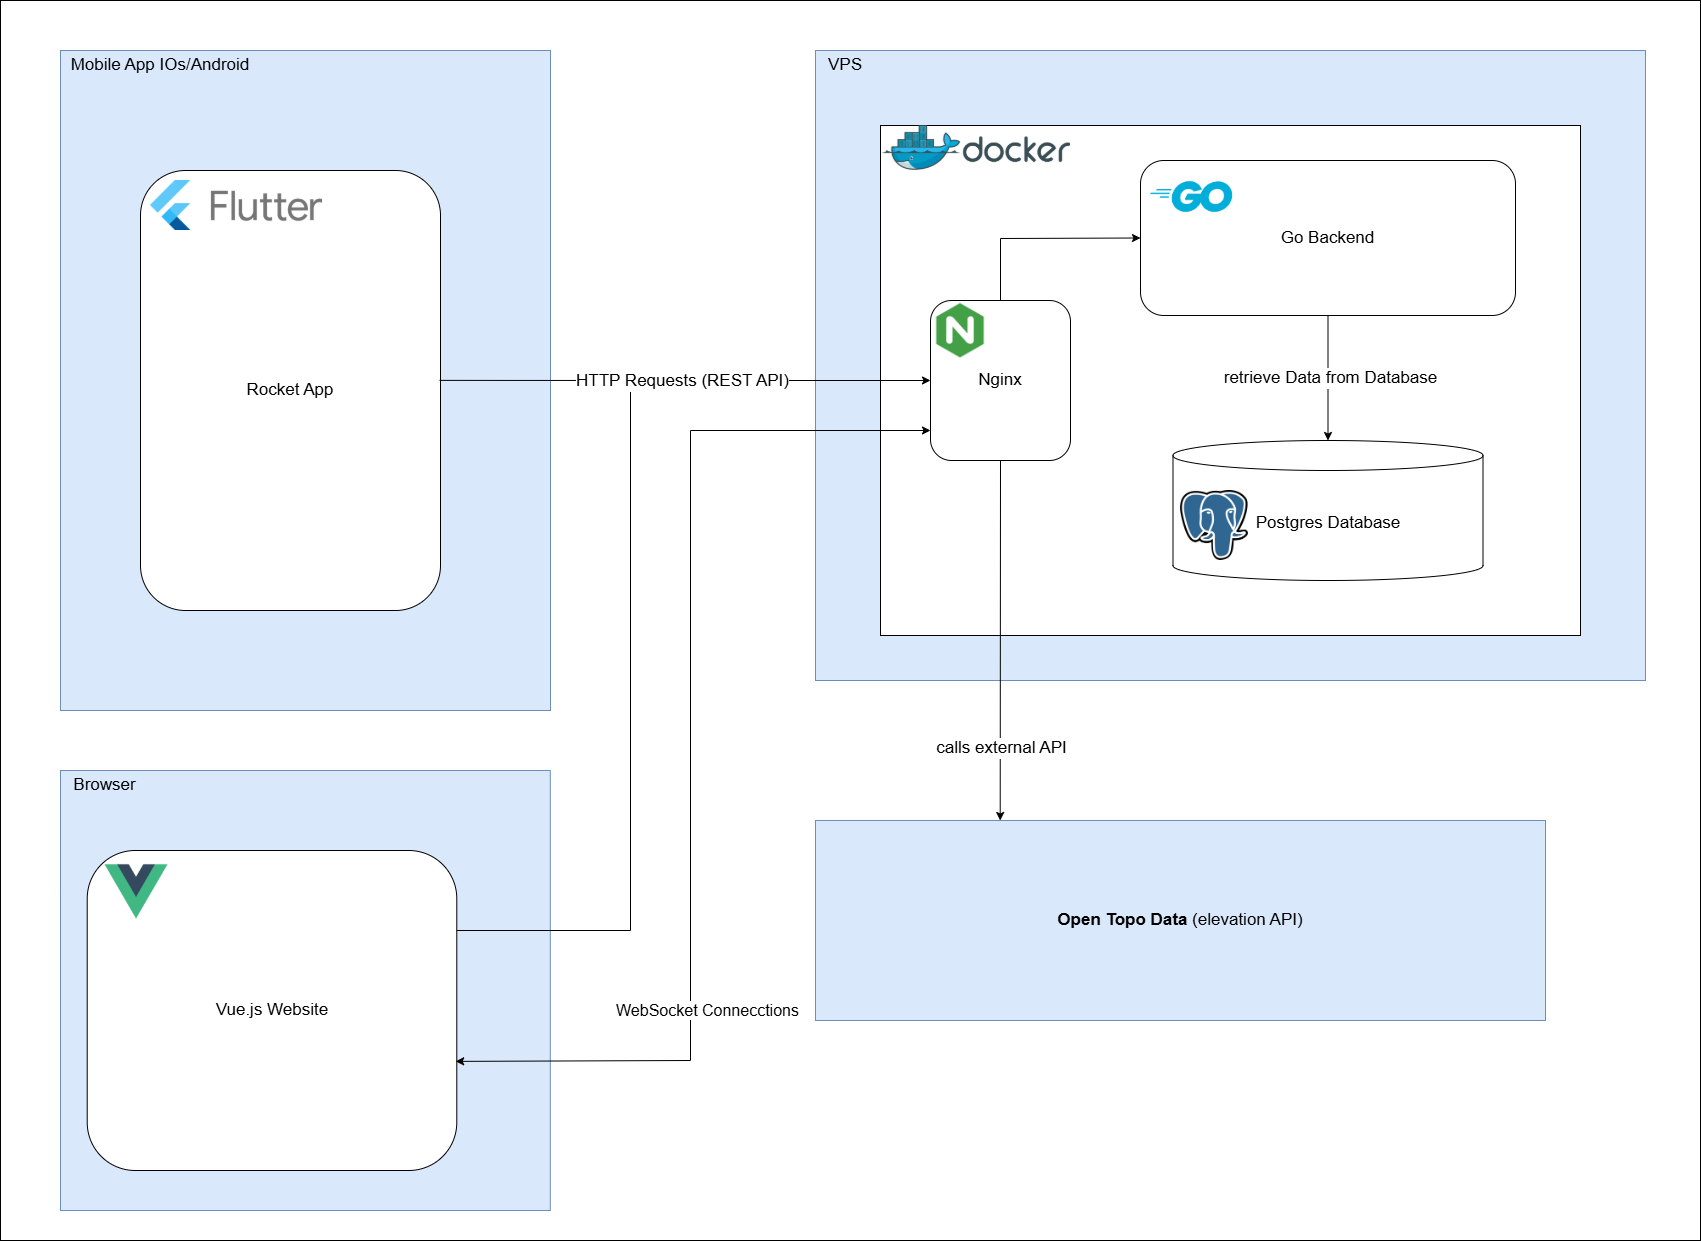
\includegraphics[width=0.95\textwidth]{images/HttpsArchitektur.png}
    \caption{Produktivarchitektur mit Docker, Nginx und HTTPS}
    \label{fig:https-architektur}
\end{figure}

\paragraph{Flutter Mobile App}
Die \textbf{Rocket App}, entwickelt mit dem Flutter Framework, läuft auf iOS und Android. Sie dient als Hauptschnittstelle für die Nutzer. Flutter wurde gewählt, weil es eine performante, plattformübergreifende Entwicklung mit einer Codebasis ermöglicht und gleichzeitig native App-Erlebnisse bietet.

Die App sendet ihre Daten  über REST-API-Aufrufe direkt an den VPS. Dabei handelt es sich um typische Aktionen wie das Hochladen von Läufen, Synchronisieren von Schritten, Highscorelisten oder das Abrufen von Challenges.

\paragraph{VPS und Containerisierung}
Der gesamte produktive Stack läuft auf einem \textbf{VPS (Virtual Private Server)}. Dies bietet volle Kontrolle über die Serverumgebung bei gleichzeitig moderaten Kosten.

Im VPS sind alle Backend-Komponenten mithilfe von \textbf{Docker} containerisiert. Docker erlaubt es, die Applikation isoliert, portabel und versionssicher zu betreiben. Dies erleichtert auch das Deployment (z.\,B. durch GitHub Actions\cite{github}) sowie die Wartung im laufenden Betrieb.

\paragraph{Nginx als Reverse Proxy}
Als erste Instanz innerhalb des VPS fungiert \textbf{Nginx}\cite{nginx}. Dieser Reverse Proxy nimmt eingehende HTTP(S)-Anfragen entgegen, kümmert sich um SSL/TLS-Verschlüsselung (z.\,B. mit Let's Encrypt) und leitet die Anfragen an den Go-Backend-Container weiter.

Die Verwendung von Nginx bringt mehrere Vorteile:
\begin{itemize}
    \item Trennung von HTTPS-Terminierung und Backend-Logik
    \item Unterstützung von statischen Dateien und Caching
    \item Flexible Weiterleitung und Lastverteilung
\end{itemize}

\paragraph{Go Backend}
Das \textbf{Go-Backend} ist der Kern der Serverlogik. Es verarbeitet alle Anfragen der Mobile App über REST-Schnittstellen. Go wurde gewählt wegen seiner hervorragenden Performance, statischen Typisierung, geringen Laufzeitanforderungen und der guten Eignung für API-Services.

Typische Funktionen des Go-Backends sind:
\begin{itemize}
    \item Verarbeiten und Speichern von Läufen, Schritten, Chats
    \item Authentifizierung und Benutzerverwaltung
    \item Bereitstellen von Geo- und Statistikdaten
\end{itemize}

\paragraph{PostgreSQL Datenbank}
Alle persistenten Daten werden in einer \textbf{PostgreSQL-Datenbank} gespeichert. PostgreSQL wurde aufgrund seiner Zuverlässigkeit, SQL-Kompatibilität und Unterstützung von Geodaten (PostGIS) ausgewählt. Es läuft ebenfalls als Docker-Container innerhalb des VPS-Netzwerks.

\paragraph{Weitere Komponenten (kurz)}
Die \textbf{Vue.js-Webseite}\cite{vuejs}, ebenfalls im Bild dargestellt, kommuniziert wie die App mit dem Backend. Zusätzlich nutzt sie WebSockets für Live-Interaktionen. Eine externe Schnittstelle – hier die \textbf{OpenTopoData API}\cite{open_topo_data} – wird vom Backend genutzt, um Höhendaten für Strecken zu ermitteln.

\paragraph{Zusammenfassung der Architekturvorteile}
\begin{itemize}
    \item \textbf{Flutter:} Plattformübergreifende Entwicklung mit nativem Look \& Feel
    \item \textbf{Go:} Hochperformant, ideal für APIs
    \item \textbf{Docker:} Portabilität, einfache Updates und Isolierung
    \item \textbf{Nginx:} Reverse Proxy für Sicherheit und Routing
    \item \textbf{PostgreSQL:} Robuste, erweiterbare SQL-Datenbank mit Geo-Support
\end{itemize}

\subsection{Lokale Entwicklungsarchitektur}
\label{sec:lokale-entwicklung}

\subsubsection{Unterschied zur Produktionsumgebung}

Die lokale Entwicklungsumgebung ist eine vereinfachte Version der Produktivarchitektur. Ziel ist es, einzelne Komponenten unabhängig testen und entwickeln zu können, ohne direkt ein Deployment auf dem VPS durchführen zu müssen.

Im Gegensatz zur vollständigen Produktionsarchitektur (siehe Abbildung \ref{fig:https-architektur}), bei der mehrere Docker-Container über einen Nginx-Reverse-Proxy orchestriert werden, wird in der lokalen Umgebung lediglich das Backend mit der zugehörigen Datenbank als \textbf{lokaler Docker-Container} betrieben.

\subsubsection{Architektur der lokalen Umgebung}
\begin{figure}[H]
    \centering
    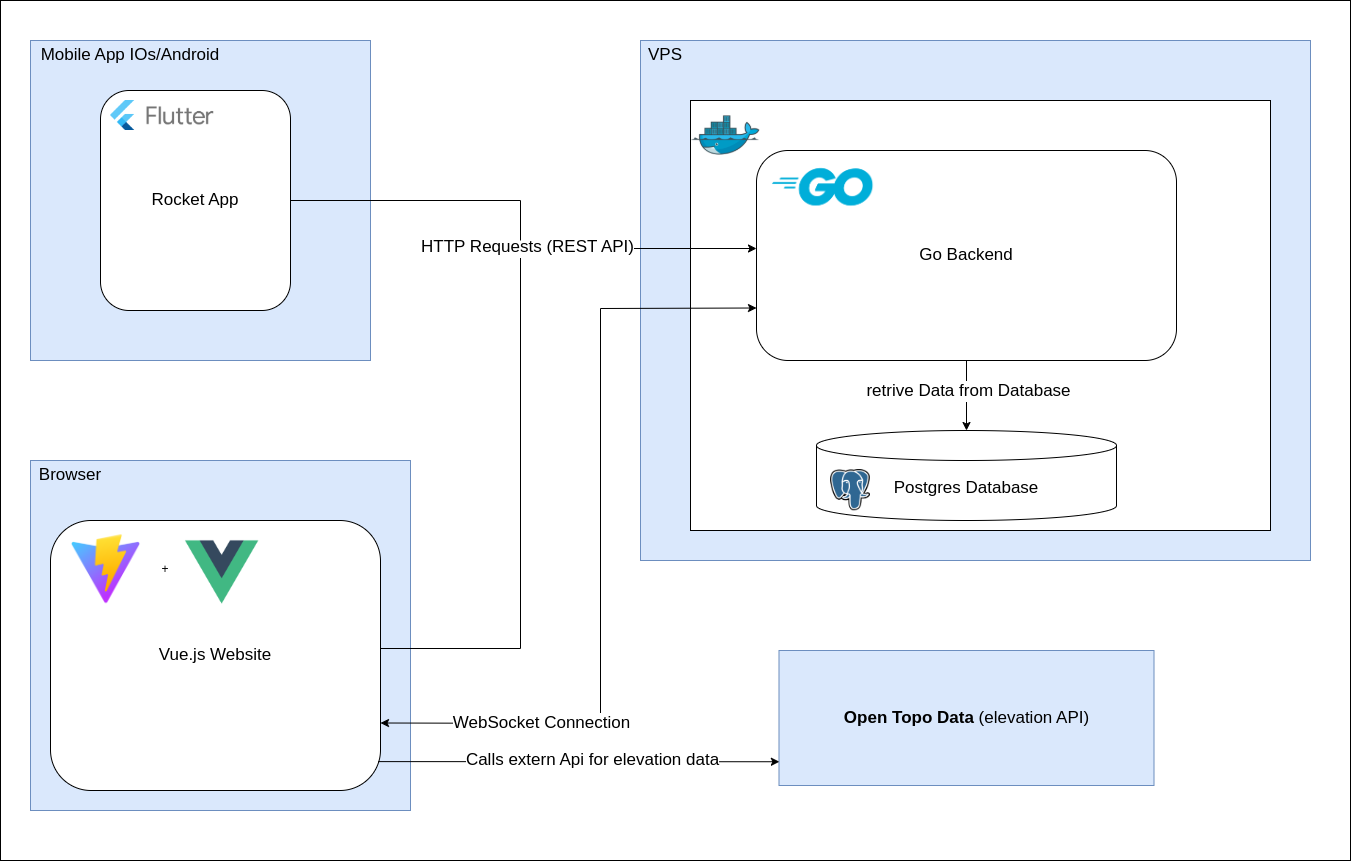
\includegraphics[width=0.9\textwidth]{images/Architecture.png}
    \caption{Lokale Entwicklungsumgebung}
    \label{fig:local-architektur}
\end{figure}

\paragraph{Backend \& Datenbank}
Das Go-Backend wird lokal in einem Docker-Container gestartet, ebenso wie eine PostgreSQL-Datenbank mit PostGIS-Erweiterung. Dadurch wird eine konsistente Entwicklungsumgebung geschaffen, die der produktiven Struktur sehr nahekommt, jedoch ohne HTTPS-Absicherung oder externe Abhängigkeiten wie Nginx.

\paragraph{Mobile App (Flutter)}
Die Mobile App kann über USB oder WLAN direkt auf einem realen Gerät installiert werden. Die Verwendung eines echten Geräts ist zwingend notwendig, da die App auf Geo-Koordinaten (GPS) und Schrittzählerdaten zugreift, welche über Gerätesensoren bereitgestellt werden. Emulatoren liefern keine oder nur ungenaue Sensorwerte und sind daher für Entwicklung und Tests ungeeignet. Für das Schrittzählen wird das Plugin \texttt{pedometer}\cite{pedometer} verwendet.

\paragraph{Web-Frontend (Vue.js + Vite)}
Das Web-Frontend basiert auf Vue.js und kann ohne Docker lokal gestartet werden. Dazu wird der \textbf{Vite Development Server}\cite{vite} verwendet. Dieser bietet schnelles Hot Reloading und ist leichtgewichtig. Eine wichtige Besonderheit ist die Verwendung eines \textbf{Proxy-Setups}, das API-Anfragen aus dem Browser zur lokal laufenden Go-API weiterleitet. Dadurch können Frontend und Backend unabhängig voneinander entwickelt werden, ohne auf ein Deployment angewiesen zu sein.

\subsection{Backend Testing}

Für das Go-Backend existiert eine umfassende Teststrategie, die auf \textbf{Integrationstests} basiert. Ziel ist es, nicht nur die einzelnen Funktionen isoliert zu testen, sondern auch das Zusammenspiel zwischen REST-Endpunkten und Datenbankabfragen realistisch zu überprüfen.

\paragraph{Verwendete Tools}
Zum Schreiben und Ausführen der Tests kommen zwei populäre Go-Testbibliotheken zum Einsatz:
\begin{itemize}
    \item \texttt{github.com/onsi/ginkgo/v2}\cite{ginkgo} – Framework für Behavior-Driven Development (BDD)
    \item \texttt{github.com/onsi/gomega}\cite{gomega} – Assertion-Bibliothek für lesbare und präzise Testausdrücke
\end{itemize}

\paragraph{Isolierte Testumgebung mit Testcontainers}
Zur Laufzeit der Tests wird mit Hilfe von \texttt{testcontainers-go}\cite{testcontainers} eine isolierte Datenbankinstanz in einem temporären Docker-Container gestartet. Diese Testdatenbank wird automatisch erstellt, mit den notwendigen Migrationsskripten versehen und nach jedem Testlauf vollständig bereinigt.

Dadurch ist sichergestellt, dass:
\begin{itemize}
    \item Jeder Test in einer identischen, kontrollierten Umgebung läuft
    \item Seiteneffekte zwischen Tests ausgeschlossen sind
    \item Produktivdaten niemals verwendet oder überschrieben werden
\end{itemize}

\paragraph{Testabdeckung}
Getestet werden:
\begin{itemize}
    \item Alle REST-Endpunkte des Backends
    \item Validierung und Fehlerfälle
    \item Alle relevanten Datenbankoperationen (CRUD)
\end{itemize}

Diese Teststrategie ermöglicht es, Änderungen im Backend schnell und sicher zu überprüfen, ohne dass manuelles Testen notwendig ist. Sie dient auch als wichtige Grundlage für zukünftige CI/CD-Pipelines.

\paragraph{Automatisierte Testausführung bei Pull Requests}
Alle Tests werden automatisch ausgeführt, sobald ein Pull Request (PR) auf den \texttt{master}-Branch erstellt wird. Dies erfolgt über eine GitHub Action, die das Test-Backend in einer isolierten Umgebung ausführt. Ein PR kann nur gemerged werden, wenn alle Tests erfolgreich durchlaufen. Dies garantiert, dass:
\begin{itemize}
    \item keine fehlerhaften Änderungen in die Hauptentwicklungslinie gelangen,
    \item alle Funktionen weiterhin wie erwartet funktionieren,
    \item die Softwarequalität über alle Sprints hinweg erhalten bleibt.
\end{itemize}


\section{ER-Modell und Datenbankarchitektur}

Die Anwendung verwendet \textbf{PostgreSQL} als relationale Datenbank, ergänzt durch zwei wichtige Erweiterungen:

\begin{itemize}
    \item \textbf{PostGIS}: Ermöglicht die Speicherung und Verarbeitung von Geodaten, insbesondere Routeninformationen als \texttt{LINESTRING}. Diese werden für Laufstrecken und geplante Routen benötigt.
    \item \textbf{pgcrypto}: Wird zur Generierung von \texttt{UUIDs} (Universally Unique Identifiers) genutzt, die als Primärschlüssel in fast allen Tabellen verwendet werden.
\end{itemize}

Die Entscheidung für UUIDs anstelle klassischer Integer-IDs beruht auf mehreren Vorteilen:
\begin{itemize}
    \item \textbf{Sicherheit}: UUIDs sind schwer zu erraten und dadurch weniger anfällig für gezielte Angriffe über ID-Inkremente.
    \item \textbf{Skalierbarkeit}: Sie ermöglichen das Erstellen von IDs über verschiedene Systeme hinweg, ohne Kollisionen befürchten zu müssen.
    \item \textbf{Unabhängigkeit von Kontexten}: Da UUIDs global eindeutig sind, kann etwa eine Laufstrecke unabhängig vom Nutzer eindeutig referenziert werden.
\end{itemize}

\begin{figure}[H]
    \centering
    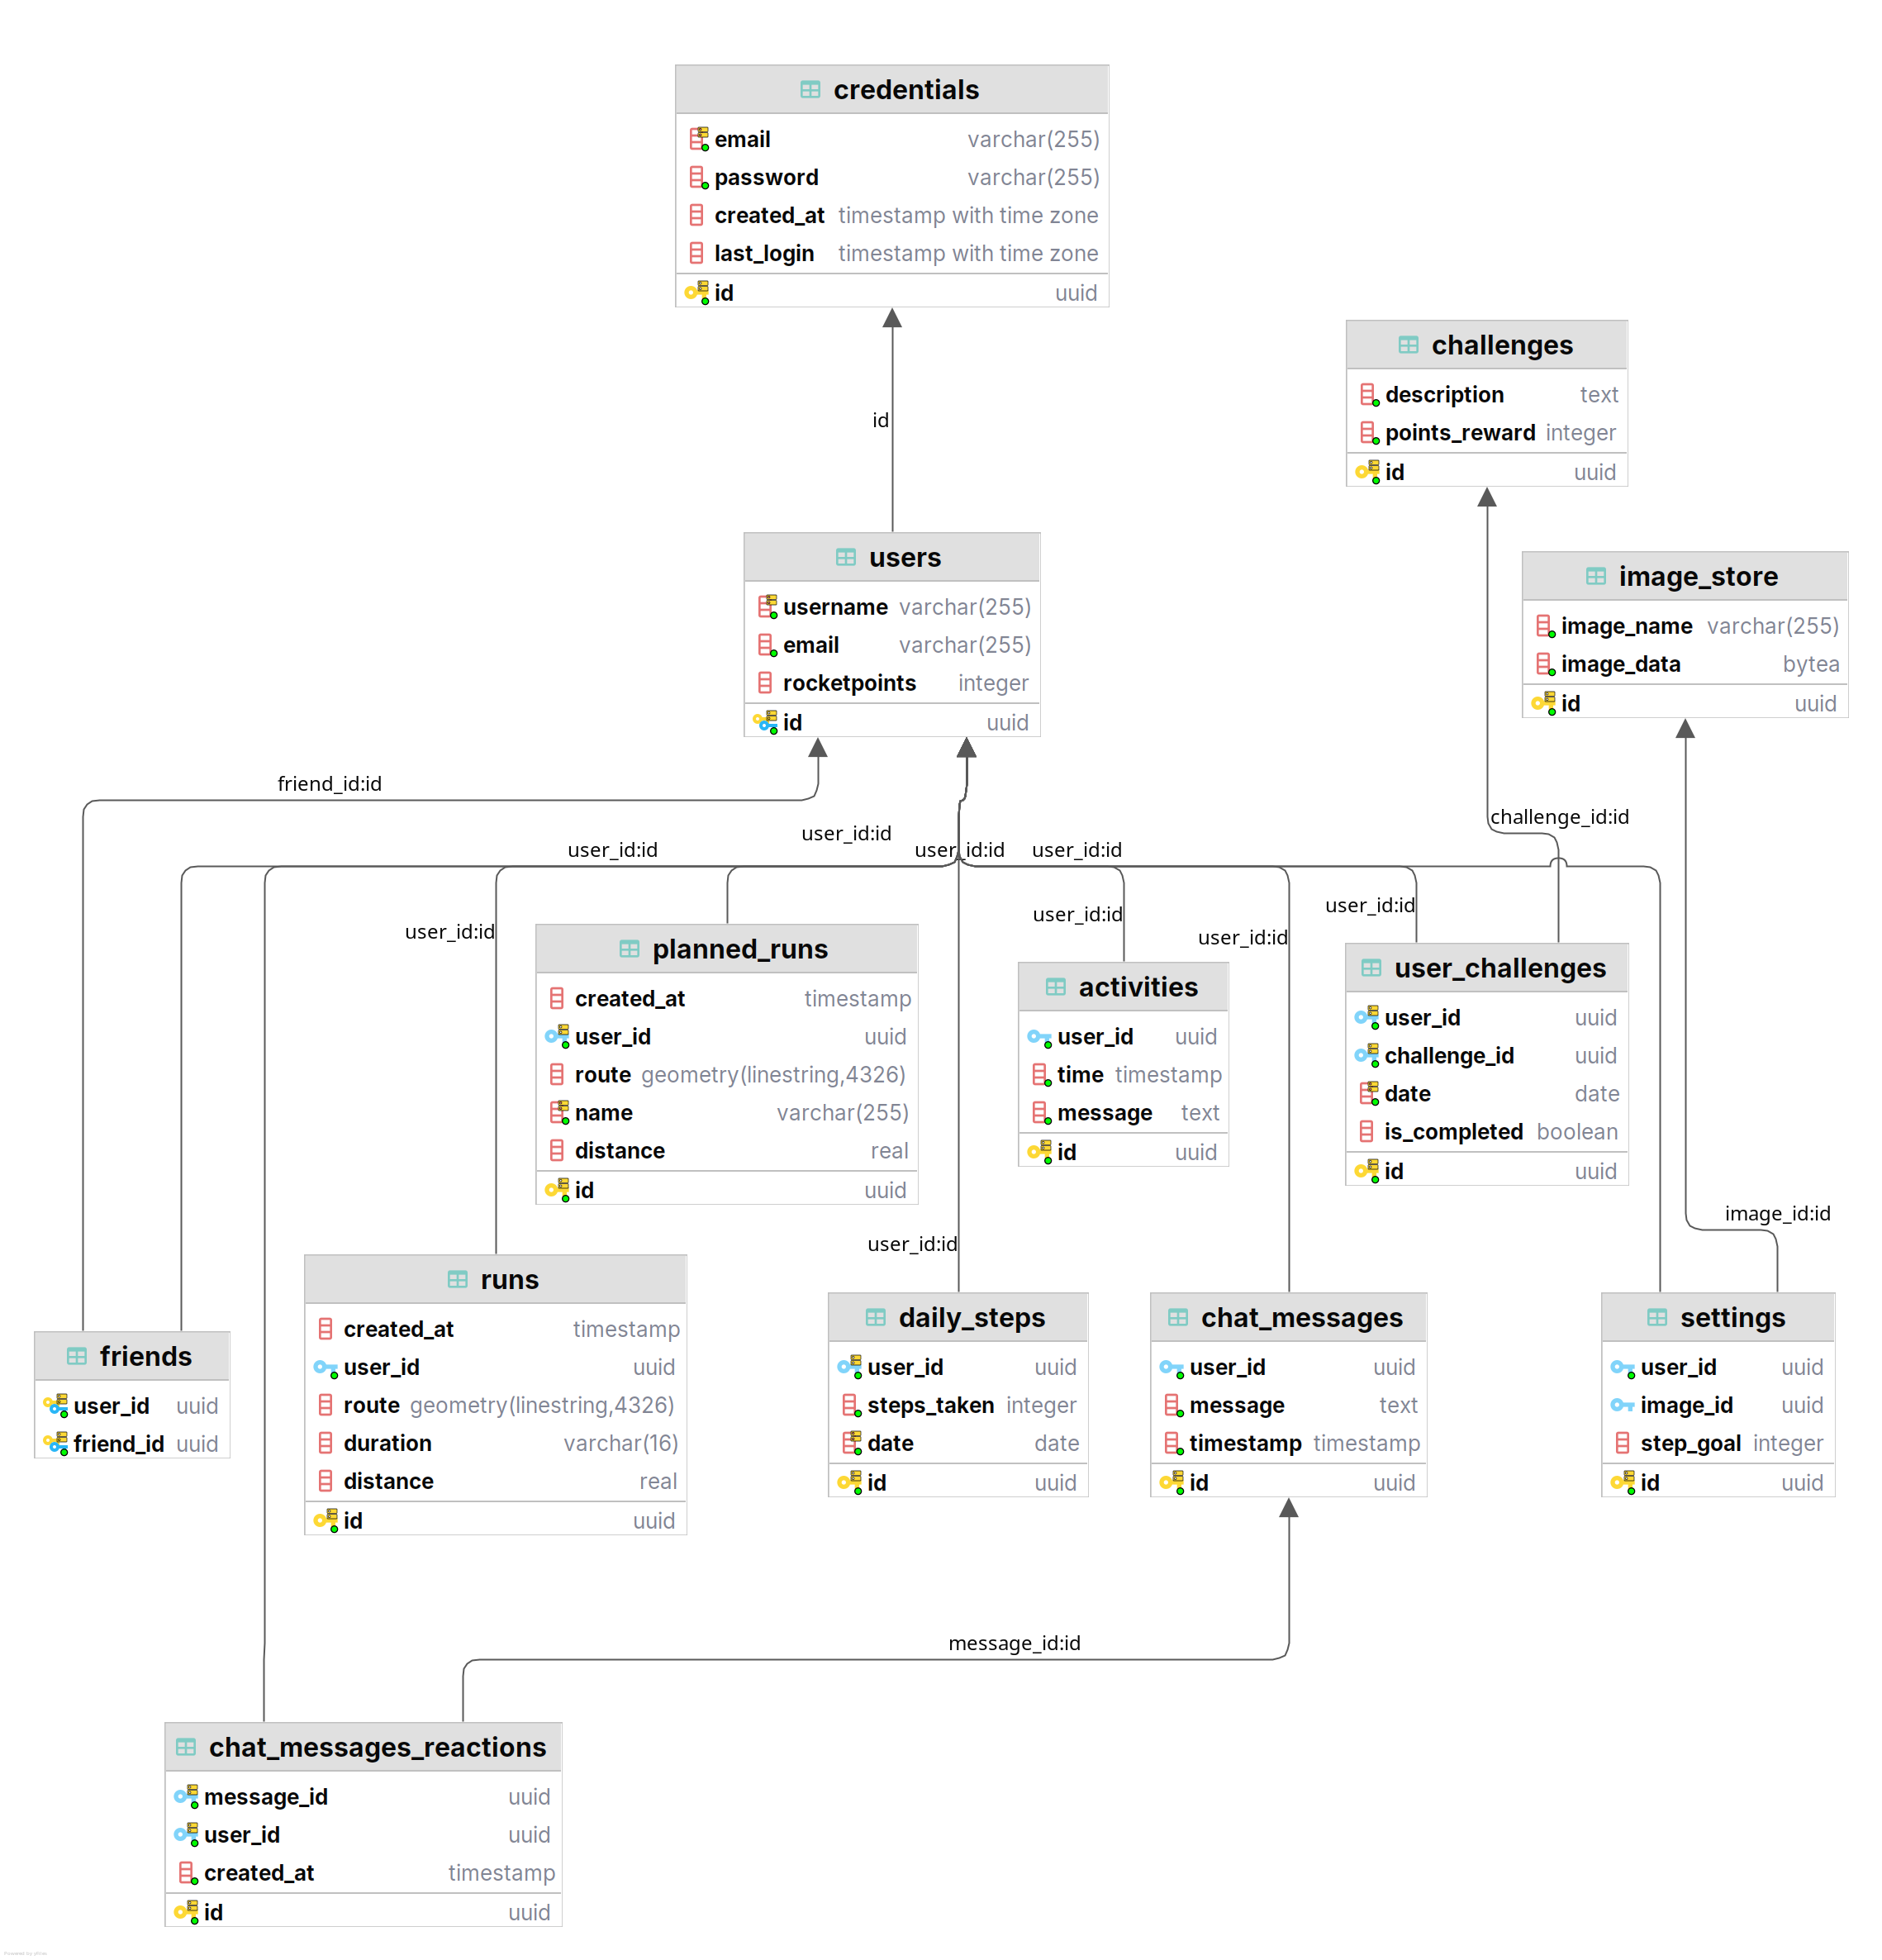
\includegraphics[width=0.8\linewidth]{images/RocketERLight.png}
    \caption{ER-Modell der Rocket-Anwendung}
\end{figure}

\begin{itemize}
    \item \textbf{users} – Zentrale Entität für Nutzer:innen der App. Enthält Username, Email und den Punktestand (Rocketpoints).
    \item \textbf{credentials} – Separat gespeicherte Zugangsdaten (E-Mail, Passwort) zur besseren Trennung von Authentifizierungs- und Nutzungsdaten.
    \item \textbf{planned\_runs} – Beinhaltet vom Nutzer vorgeplante Routen (mit Geometrie), Name und Ziel-Distanz. Essentiell für die Trainingsplanung.
    \item \textbf{runs} – Tatsächlich durchgeführte Läufe, ebenfalls mit Geodaten, Distanz und Dauer. Grundlage für Fortschrittsverfolgung.
    \item \textbf{daily\_steps} – Aggregierte tägliche Schrittzahlen pro Nutzer, oft durch Sensorschnittstellen (z.\,B. Mobilgerät) geliefert.
    \item \textbf{activities} – Logbuch-Funktion für allgemeine Nutzeraktionen. Enthält Textnachrichten und Zeitstempel.
    \item \textbf{friends} – Bidirektionale Freundschaften zwischen Nutzer:innen. Erlaubt soziales Tracking und Interaktion.
    \item \textbf{challenges} – Vorgedefinierte Herausforderungen mit Beschreibung und Punktebelohnung.
    \item \textbf{user\_challenges} – Relationstabelle zwischen Nutzer:innen und Herausforderungen, inkl. Statusinformationen wie \texttt{is\_completed}.
    \item \textbf{settings} – Benutzerbezogene Konfigurationen, insbesondere Zielwerte wie Schrittanzahl oder Profilbild.
    \item \textbf{image\_store} – Speicherung binärer Bilddaten (z.\,B. Avatare, Challenge-Bilder). Gekoppelt an andere Tabellen über \texttt{image\_id}.
    \item \textbf{chat\_messages} – Ermöglicht einfache Nachrichten zwischen Nutzer:innen. Repräsentiert den sozialen Aspekt der App.
    \item \textbf{chat\_messages\_reactions} – Erweiterung für Reaktionen (z.\,B. Emojis) auf Chatnachrichten. Enthält Zeitstempel und Verweis auf Nutzer:in.
\end{itemize}

Alle Relationen sind über \texttt{uuid}-Fremdschlüssel miteinander verknüpft, was eine klare logische Trennung und Erweiterbarkeit des Systems unterstützt. Die Kombination aus Geodaten, sozialen Funktionen und gamifizierter Nutzerinteraktion bildet das Rückgrat der Applikation.


\section{Authentifizierung und User Validierung}

Für die Authentifizierung und Validierung der Nutzer setzen wir auf JSON Web Tokens (JWT) \cite{jwt}. JWT ermöglicht eine sichere und effiziente Methode, um Benutzeridentitäten zwischen Client und Server zu verifizieren, ohne bei jeder Anfrage die Datenbank abfragen zu müssen.

Der große Vorteil von JWT liegt darin, dass alle nötigen Informationen in einem signierten Token gebündelt sind, das sowohl Integrität als auch Authentizität gewährleistet. Dies reduziert die Serverlast und ermöglicht gleichzeitig eine skalierbare und stateless-Authentifizierung.

In unserer Architektur unterscheiden wir die Handhabung des Tokens zwischen App und Web:

\begin{itemize}
    \item \textbf{Mobile App:} Hier wird der JWT nach erfolgreichem Login sicher im \texttt{SecureStorage} gespeichert, um ihn bei nachfolgenden API-Anfragen im Header mitzuschicken. Das Plugin \texttt{flutter\_secure\_storage}\cite{flutter_secure_storage} gewährleistet, dass der Token verschlüsselt und vor unbefugtem Zugriff geschützt ist. Ein Beispiel zur Speicherung sieht folgendermaßen aus:

\begin{lstlisting}[language=Dart, caption=Speichern des JWT im Secure Storage]
await _storage.write(key: 'jwt_token', value: loginResponse.token);
\end{lstlisting}

    \item \textbf{Webanwendung:} Im Browser wird der JWT als HTTP-Cookie verwaltet. Dies ermöglicht eine einfache automatische Übertragung bei Anfragen und reduziert die Notwendigkeit, den Token manuell im Header zu setzen.
\end{itemize}

Alle API-Endpunkte außer \texttt{/login} und \texttt{/register} sind als \textit{protected routes} konfiguriert. Das bedeutet, dass jede Anfrage an diese Endpunkte nur mit einem gültigen JWT im Header akzeptiert wird. Auf diese Weise verhindern wir, dass unautorisierte Nutzer auf geschützte Daten zugreifen können.

Beim Fehlen eines gültigen Tokens oder bei einem abgelaufenen Token wird der Zugriff verweigert und ein entsprechender Fehler (z.B. HTTP 401 Unauthorized) zurückgegeben. Dieses Vorgehen stellt sicher, dass sensible Daten und Funktionen nur authentifizierten Benutzern zugänglich sind.

Der Authentifizierungs-Workflow ist in Abbildung~\ref{fig:validation-workflow} schematisch dargestellt.

\begin{figure}[H]
    \centering
    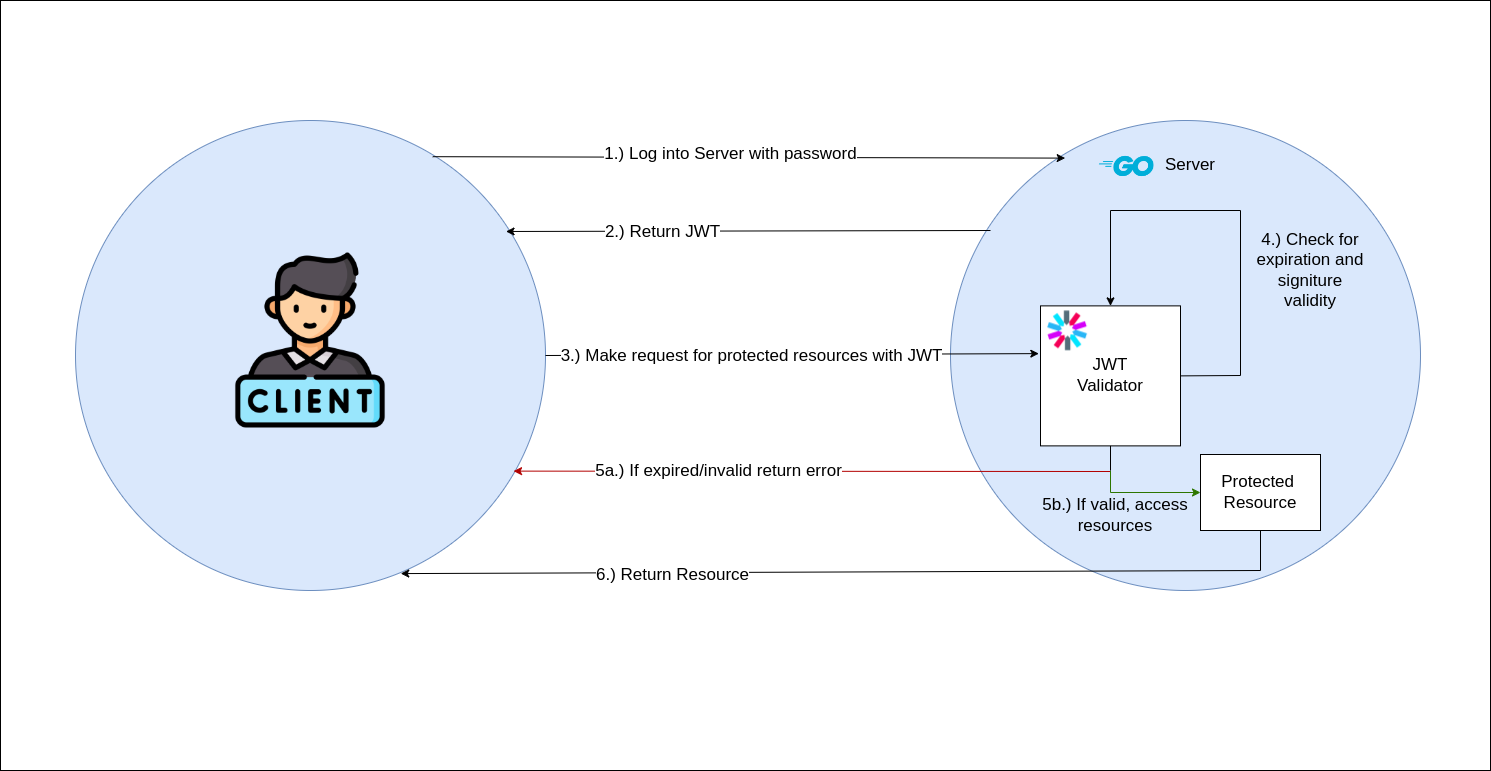
\includegraphics[width=0.9\textwidth]{images/ValidationWorkflow.png}
    \caption{Workflow der Nutzer-Validierung mittels JWT}
    \label{fig:validation-workflow}
\end{figure}

Die Entscheidung für JWT fiel aufgrund der folgenden Gründe:
\begin{itemize}
    \item \textbf{Skalierbarkeit:} Da JWT stateless ist, muss der Server keine Sitzungsdaten speichern, was die Skalierung der Anwendung erleichtert.
    \item \textbf{Sicherheit:} Durch die Signatur des Tokens wird sichergestellt, dass der Token nicht manipuliert wurde.
    \item \textbf{Flexibilität:} JWT kann problemlos in verschiedenen Client-Typen (Mobile, Web) genutzt werden und erlaubt verschiedene Nutzlasten (Claims).
\end{itemize}

Durch diese Implementierung gewährleisten wir eine sichere, performante und flexible Authentifizierung, die sich nahtlos in unsere Cross-Plattform-Lösung integriert.

\section{Backend}

\subsection{Endpunkte}

Im Folgenden werden alle Backend-Endpunkte der Rocket App API dokumentiert. Die API ist unter dem Prefix \texttt{/api/v1} verfügbar. Für alle \texttt{/protected}-Routen ist eine Authentifizierung erforderlich (JWT im Header).
Der Header für fast alle protected Endpunkte sieht so aus: 
    \textbf{Headers:}
    \begin{itemize}
        \item \texttt{Authorization: Bearer <token>}
        \item \texttt{Content-Type: application/json}
    \end{itemize}

\subsubsection{Authentication}

\begin{itemize}[leftmargin=1.5cm]
    \item[\textbf{POST}] \texttt{/api/v1/register} \\
    Registriert einen neuen Nutzer.

    \textbf{Request Body:}
    \begin{lstlisting}[language=json]
{
  "email": "user@example.com",
  "username": "username",
  "password": "securepassword"
}
    \end{lstlisting}

\item[\textbf{POST}] \texttt{/api/v1/login} \\
Loggt einen Nutzer ein und gibt ein JWT zurück.

\textbf{Request Body:}
\begin{lstlisting}[language=json]
{
  "email": "user@example.com",
  "password": "securepassword"
}
\end{lstlisting}

\textbf{Response Body:}
\begin{lstlisting}[language=json]
{
  "token": "eyJhbGciOiJIUzI1NiIsInR5cCI6IkpXVCJ9..."
}
\end{lstlisting}

\textbf{Hinweis:}
\begin{itemize}
  \item Der JWT wird sowohl im Response-Body zurückgegeben als auch als \texttt{HttpOnly}, \texttt{Secure}-Cookie mit dem Namen \texttt{jwt\_token} gesetzt.
  \item Die Lebensdauer des Cookies beträgt 72 Stunden.
  \item Das Cookie ist nur über HTTPS übertragbar und nicht über JavaScript auslesbar.
\end{itemize}

    \item[\textbf{POST}] \texttt{/api/v1/logout} \\
    Entfernt das JWT als Cookie vom Nutzer.

\item[\textbf{GET}] \texttt{/api/v1/protected/} \\
Überprüfe, ob ein User angemeldet ist und einen validen JWT besitzt.
\end{itemize}



\subsubsection{User-Endpunkte}

\begin{itemize}

\item[\textbf{GET}] \texttt{/api/v1/user} \\
Gibt die Informationen des aktuell eingeloggten Nutzers zurück.

\textbf{Response Body:}
\begin{lstlisting}[language=json]
{
  "id": "UUID",
  "username": "exampleuser",
  "email": "user@example.com",
  "rocket_points": 120
}
\end{lstlisting}

\item[\textbf{DELETE}] \texttt{/api/v1/user} \\
Löscht den aktuell eingeloggten Nutzer.

\item[\textbf{GET}] \texttt{/api/v1/user/:name} \\
Gibt die Informationen zu einem Nutzer anhand des Usernames zurück (inkl. Bilddaten, falls vorhanden).

\textbf{Response Body:}
\begin{lstlisting}[language=json]
{
  "id": "UUID",
  "username": "johndoe",
  "email": "john@example.com",
  "rocket_points": 100,
  "image_name": "profile.png",
  "image_data": "Base64EncodedData"
}
\end{lstlisting}

\item[\textbf{POST}] \texttt{/api/v1/user/statistics} \\
Gibt die Schrittstatistik eines Nutzers für die letzten 7 Tage zurück. Wenn kein Body angegeben ist, wird der eingeloggte Nutzer verwendet.

\textbf{Request Body (optional):}
\begin{lstlisting}[language=json]
{
  "id": "UUID"
}
\end{lstlisting}

\textbf{Response Body:}
\begin{lstlisting}[language=json]
[
  {
    "day": "2025-06-24",
    "steps": 4321
  },
  ...
  {
    "day": "2025-06-18",
    "steps": 6200
  }
]
\end{lstlisting}

\item[\textbf{POST}] \texttt{/api/v1/user/image} \\
Lädt das Profilbild eines Nutzers (eigener oder über ID im Body).

\textbf{Request Body (optional):}
\begin{lstlisting}[language=json]
{
  "user_id": "UUID"
}
\end{lstlisting}

\textbf{Response Body:}
\begin{lstlisting}[language=json]
{
  "username": "johndoe",
  "name": "profile.jpg",
  "mime_type": "image/jpeg",
  "data": "Base64EncodedImage"
}
\end{lstlisting}

\item[\textbf{GET}] \texttt{/api/v1/user/rocketpoints} \\
Gibt die RocketPoints des eingeloggten Nutzers zurück.

\textbf{Response Body:}
\begin{lstlisting}[language=json]
{
  "rocket_points": 125
}
\end{lstlisting}

\item[\textbf{GET}] \texttt{/api/v1/users} \\
Gibt eine Liste aller Nutzer mit ihren Daten und Bildern zurück.

\textbf{Response Body:}
\begin{lstlisting}[language=json]
[
  {
    "id": "UUID",
    "username": "johndoe",
    "email": "john@example.com",
    "rocket_points": 100,
    "steps": 2345,
    "image_name": "profile.jpg",
    "image_data": "Base64EncodedImage"
  },
  ...
]
\end{lstlisting}

    \item[\textbf{POST}] \texttt{/api/v1/protected/updateSteps} \\
    Aktualisiert die Schrittanzahl des aktuellen Nutzers.

    \textbf{Request Body:}
    \begin{lstlisting}[language=json]
{
  "steps": 1234
}
    \end{lstlisting}
\end{itemize}


\subsubsection{Settings}

\begin{itemize}[leftmargin=1.5cm]
    \item[\textbf{GET}] \texttt{/api/v1/protected/settings} \\
    Gibt aktuelle Benutzereinstellungen zurück.

    \item[\textbf{POST}] \texttt{/api/v1/protected/settings/step-goal} \\
    Aktualisiert das Schrittziel des Nutzers.

    \textbf{Request Body:}
    \begin{lstlisting}[language=json]
{
  "stepGoal": 8000
}
    \end{lstlisting}

    \item[\textbf{POST}] \texttt{/api/v1/protected/settings/image} \\
    Aktualisiert das Profilbild eines authentifizierten Benutzers.

    \textbf{Headers:}
    \begin{itemize}
        \item \texttt{Authorization: Bearer <token>}
        \item \texttt{Content-Type: multipart/form-data}
    \end{itemize}

    \textbf{Form-Data Felder:}
    \begin{itemize}
        \item \texttt{image} -- Bilddatei (JPEG, PNG etc.)
    \end{itemize}

    \textbf{Beispielanfrage mit \texttt{curl}:}
    \begin{lstlisting}
curl -X POST http://localhost:8080/api/v1/protected/settings/image \
  -H "Authorization: Bearer <your_jwt>" \
  -F "image=@profile.jpg"
    \end{lstlisting}

    \item[\textbf{DELETE}] \texttt{/api/v1/protected/settings/image} \\
    Löscht das aktuelle Profilbild.

    \item[\textbf{POST}] \texttt{/api/v1/protected/settings/userinfo} \\
    Aktualisiert die Benutzerinformationen wie Name, E-Mail oder Passwort. Es können beliebige Felder gesendet werden – sie sind alle optional. Die Passwortänderung erfordert das aktuelle Passwort.

    \textbf{Request Body:}
    \begin{lstlisting}[language=json]
{
  "name": "Max Mustermann",
  "email": "max@example.com",
  "currentPassword": "oldpass123",
  "newPassword": "newpass456"
}
    \end{lstlisting}
\end{itemize}

\subsubsection{Challenges}

\begin{itemize}[leftmargin=1.5cm]
    \item[\textbf{GET}] \texttt{/api/v1/protected/challenges/new} \\
    Gibt die aktuellen täglichen Challenges zurück.

    \item[\textbf{POST}] \texttt{/api/v1/protected/challenges/complete} \\
    Markiert eine Challenge als abgeschlossen.

    \textbf{Request Body:}
    \begin{lstlisting}[language=json]
{
  "challenge_id": "uuid-abc...",
  "rocket_points": 20
}
    \end{lstlisting}

    \item[\textbf{GET}] \texttt{/api/v1/protected/challenges/progress} \\
    Gibt den Fortschritt der täglichen Challenges zurück.

    \item[\textbf{POST}] \texttt{/api/v1/protected/challenges/invite} \\
    Lädt einen Freund zu einer Challenge ein.

    \textbf{Request Body:}
    \begin{lstlisting}[language=json]
{
  "challenge_id": "ccf4fe0e-002f-4fbd-80d6-0670db8a979b",
  "friend_id": "80c2f290-7644-4f76-9d87-cb5d39501c42"
}
    \end{lstlisting}
\end{itemize}

\subsubsection{Ranking}

\begin{itemize}[leftmargin=1.5cm]
    \item[\textbf{GET}] \texttt{/api/v1/protected/ranking/users} \\
    Gibt eine Liste der Top 100 Nutzer nach Rocket Points zurück (globales Ranking).

    \textbf{Response Body:}
    \begin{lstlisting}[language=json]
[
  {
    "id": "9cfa8b97-7adf-4d2b-b408-882db5adf511",
    "username": "john_doe",
    "email": "john@example.com",
    "rocketPoints": 320,
    "imageName": "avatar.png",
    "imageData": "<base64-encoded>",
    "steps": 0
  },
  ...
]
    \end{lstlisting}

    \item[\textbf{GET}] \texttt{/api/v1/protected/ranking/friends} \\
    Gibt das Ranking der Freunde des Nutzers nach Rocket Points zurück.

    \textbf{Response Body:}
    \begin{lstlisting}[language=json]
[
  {
    "id": "8ab7f178-e0e3-4cfc-a8b2-20b420b8f2ee",
    "username": "jane_doe",
    "email": "jane@example.com",
    "rocketPoints": 250,
    "imageName": "jane.png",
    "imageData": "<base64-encoded>",
    "steps": 0
  },
  ...
]
    \end{lstlisting}
\end{itemize}

\subsubsection{Friends}

\begin{itemize}[leftmargin=1.5cm]
    \item[\textbf{GET}] \texttt{/api/v1/protected/friends} \\
    Gibt eine Liste aller Freunde des angemeldeten Nutzers mit Bild, RocketPoints und aktuellen Schritten zurück.

    \textbf{Response Body:}
    \begin{lstlisting}[language=json]
[
  {
    "id": "user-uuid-1",
    "username": "alice",
    "email": "alice@example.com",
    "rocketPoints": 230,
    "imageName": "avatar.png",
    "imageData": "<base64-encoded>",
    "steps": 5374
  },
  ...
]
    \end{lstlisting}

    \item[\textbf{POST}] \texttt{/api/v1/protected/friends/add} \\
    Fügt einen neuen Freund anhand des Benutzernamens hinzu.

    \textbf{Request Body:}
    \begin{lstlisting}[language=json]
{
  "friend_name": "bob"
}
    \end{lstlisting}


    \item[\textbf{DELETE}] \texttt{/api/v1/protected/friends/:name} \\
    Entfernt einen Freund anhand des Benutzernamens.


    \item[\textbf{GET}] \texttt{/api/v1/protected/following/:id} \\
    Gibt eine Liste aller Nutzer zurück, denen der Benutzer mit der angegebenen UUID folgt.

    \textbf{Response Body:}
    \begin{lstlisting}[language=json]
[
  {
    "id": "user-uuid-2",
    "username": "charlie",
    "email": "charlie@example.com",
    "rocketPoints": 180,
    "imageName": "charlie.png",
    "imageData": "<base64-encoded>",
    "steps": 0
  },
  ...
]
    \end{lstlisting}

    \item[\textbf{GET}] \texttt{/api/v1/protected/followers/:id} \\
    Gibt eine Liste aller Nutzer zurück, die dem Benutzer mit der angegebenen UUID folgen.

    \textbf{Response Body:}
    \begin{lstlisting}[language=json]
[
  {
    "id": "user-uuid-3",
    "username": "david",
    "email": "david@example.com",
    "rocketPoints": 160,
    "imageName": "david.png",
    "imageData": "<base64-encoded>",
    "steps": 0
  },
  ...
]
    \end{lstlisting}
\end{itemize}

\subsubsection{Runs}

\begin{itemize}[leftmargin=1.5cm]

  \item[\textbf{POST}] \texttt{/api/v1/protected/runs} \\
  Lädt eine neue Laufaktivität hoch.

  \textbf{Request Body:}
  \begin{lstlisting}[language=json]
{
  "route": "LINESTRING(....)",
  "duration": "25m30s",
  "distance": 5.23
}
  \end{lstlisting}

  \item[\textbf{GET}] \texttt{/api/v1/protected/runs} \\
  Gibt alle hochgeladenen Läufe des authentifizierten Nutzers zurück.

  \textbf{Response Body (200 OK):}
  \begin{lstlisting}[language=json]
[
  {
    "id": "run-uuid-1",
    "route": "LINESTRING(....)",,
    "duration": "25m30s",
    "distance": 5.23
  },
  ...
]
  \end{lstlisting}

  \item[\textbf{DELETE}] \texttt{/api/v1/protected/runs/:id} \\
  Löscht den Lauf mit der angegebenen UUID.

  \item[\textbf{POST}] \texttt{/api/v1/protected/runs/plan} \\
  Plant einen zukünftigen Lauf.

  \textbf{Request Body:}
  \begin{lstlisting}[language=json]
{
  "route": "LINESTRING(....)",
  "name": "Morning Run",
  "distance": 7.5
}
  \end{lstlisting}

  \item[\textbf{GET}] \texttt{/api/v1/protected/runs/plan} \\
  Gibt alle geplanten Läufe des authentifizierten Nutzers zurück.

  \textbf{Response Body (200 OK):}
  \begin{lstlisting}[language=json]
[
  {
    "id": "planned-run-uuid-1",
    "route": "LINESTRING(....)",
    "name": "Morning Run",
    "distance": 7.5
  },
  ...
]
  \end{lstlisting}

  \item[\textbf{DELETE}] \texttt{/api/v1/protected/runs/plan/:id} \\
  Löscht den geplanten Lauf mit der angegebenen UUID.

\end{itemize}

\subsubsection{Aktivitäten und Chat}

\begin{itemize}[leftmargin=1.5cm]

  \item[\textbf{GET}] \texttt{/api/v1/protected/activities} \\
  Gibt Aktivitäten des aktuellen Benutzers sowie seiner Freunde zurück. Die Antwort enthält optional Benutzerbilder.

  \begin{itemize}
    \item \textbf{Response:}
\begin{lstlisting}[language=json]
{
  "username": "johndoe",
  "activities": [
    {
      "name": "johndoe",
      "time": "2025-06-25T13:14:00Z",
      "message": "Completed a 5.00 km run in 28 minutes",
      "imageName": "profile.jpg",
      "imageType": "image/jpeg",
      "imageData": "base64-encoded-data"
    },
    ...
  ]
}
\end{lstlisting}
  \end{itemize}

  \item[\textbf{GET}] \texttt{/api/v1/protected/chat/history} \\
  Gibt alle bisherigen Chatnachrichten des Benutzers zurück.

  \begin{itemize}
    \item \textbf{Response:}
\begin{lstlisting}[language=json]
{
  "messages": [
    {
      "id": "uuid",
      "username": "alice",
      "message": "Hello, everyone!",
      "timestamp": "2025-06-25T12:30:00Z",
      "reactions": 3,
      "hasReacted": true
    },
    ...
  ]
}
\end{lstlisting}
  \end{itemize}

  \item[\textbf{GET}] \texttt{/api/v1/protected/ws/chat} \\
  Öffnet eine WebSocket-Verbindung für den globalen Chat.

  \begin{itemize}
    \item \textbf{WebSocket-Nachrichtenformat (Text, JSON):}
\begin{lstlisting}[language=json]
{
  "username": "bob",
  "message": "Let's go for a run!",
  "timestamp": "2025-06-25T13:40:00Z"
}
\end{lstlisting}
    \item Reaktionen und Nutzerverbindungen werden serverseitig verwaltet. Nachrichten werden über einen \texttt{ChatHub} verteilt.
  \end{itemize}

\end{itemize}

\subsection{Docker Container}

Die gesamte Anwendung besteht aus mehreren Docker-Containern, die über ein gemeinsames Netzwerk \texttt{blueprint} verbunden sind. Das Setup basiert auf \texttt{docker-compose} und ist für den produktiven Einsatz auf einem VPS optimiert. Alle internen Services sind sauber voneinander getrennt und verwenden eigene Images.

\begin{itemize}
  \item[\textbf{backend}] \texttt{zephiron/rocket-backend:latest} \\
  Dieser Container stellt die REST-API der Anwendung bereit. Er ist in Go implementiert und verbindet sich mit der PostgreSQL-Datenbank. Die wichtigsten Umgebungsvariablen beinhalten z.\,B. \texttt{JWT\_SECRET} und \texttt{DATABASE\_URL}. Das Image wird vorab gebaut und auf Docker Hub veröffentlicht, um die Build-Zeit auf dem Server zu sparen.

  \item[\textbf{frontend}] \texttt{zephiron/rocket-website:latest} \\
  Die statische Website mit Vue.js läuft in einem eigenen Container und wird ebenfalls über Docker Hub bereitgestellt. Auch hier wird durch die vorgefertigten Images eine schnelle und ressourcensparende Bereitstellung ermöglicht.

  \item[\textbf{postgres}] \texttt{postgis/postgis:latest} \\
  Die Datenbank verwendet PostgreSQL mit der PostGIS-Erweiterung für mögliche geographische Erweiterungen. Persistenz wird über ein Docker-Volume gewährleistet. Ein Healthcheck stellt sicher, dass der Container erst als \textit{ready} markiert wird, wenn Verbindungen angenommen werden können.

  \item[\textbf{migrate}] \texttt{migrate/migrate} \\
  Dieser Container führt automatisch Migrationen beim Start aus. Er nutzt das offizielle \texttt{migrate} CLI-Tool und greift über ein Volume auf die lokalen Migrationsdateien zu.

  \item[\textbf{reverse-proxy}] \texttt{nginx:1.27-alpine} \\
  Dieser NGINX-Container agiert als Reverse-Proxy für alle eingehenden HTTP(S)-Anfragen. Er leitet:
  \begin{itemize}
    \item \texttt{/api/v1/} an das \textbf{Backend} weiter (inkl. WebSocket-Unterstützung)
    \item \texttt{/elevation-api/} an den externen Service \texttt{https://api.opentopodata.org}
    \item alle anderen Pfade an das \textbf{Frontend}
  \end{itemize}

  Besonders hervorzuheben ist, dass der Reverse-Proxy \textbf{HTTPS über Let's Encrypt-Zertifikate} unterstützt. Alle Anfragen auf Port 80 werden automatisch auf HTTPS (Port 443) umgeleitet. Die Zertifikate werden lokal im Container gemountet:

  \begin{lstlisting}
  ssl_certificate /etc/letsencrypt/live/rocket-app.social/fullchain.pem;
  ssl_certificate_key /etc/letsencrypt/live/rocket-app.social/privkey.pem;
  \end{lstlisting}

  Dadurch ist sichergestellt, dass die gesamte Anwendung über eine verschlüsselte Verbindung (HTTPS) erreichbar ist — ein wichtiger Sicherheitsaspekt im Produktivbetrieb.
\end{itemize}

\vspace{1em}

\textbf{Vorteil der Build-Strategie:}  
Da die \texttt{backend}- und \texttt{frontend}-Images bereits lokal entwickelt und anschließend auf Docker Hub (\texttt{zephiron/*}) veröffentlicht werden, muss der VPS keine eigenen Build-Prozesse ausführen. Dies spart sowohl Speicher als auch CPU-Zeit und minimiert mögliche Build-Fehler während der Bereitstellung. Die Container können dadurch direkt per \texttt{docker pull} geladen und gestartet werden.


\section{Handy App}
\subsection{Foreground Task}

Die App verwendet das Flutter-Plugin \texttt{flutter\_foreground\_task}\cite{flutter_foreground_task}, um dauerhaft im Vordergrund bzw. Hintergrund Schrittzahlen zu erfassen und regelmäßig an das Backend zu senden. Dies ist vor allem unter Android notwendig, da das Betriebssystem Hintergrundprozesse stark einschränkt und andernfalls wichtige Trackingdaten verloren gehen könnten.

Die Foreground Task besteht aus zwei getrennten Instanzen, welche in unterschiedlichen Isolates (Flutter-Threads) laufen. Diese kommunizieren nicht direkt über Speicher, sondern über Ports:

\begin{itemize}[leftmargin=1.5em]
    \item \textbf{Hauptanwendung (Main Isolate)}: Dies ist der Hauptthread, in dem auch die Benutzeroberfläche läuft. Dort wird der Foreground-Task initialisiert und gestartet.
\end{itemize}

\begin{lstlisting}[language=Dart, caption=Initialisierung des Foreground Task]
FlutterForegroundTask.initCommunicationPort();
_initService();
await _startService();
\end{lstlisting}

\begin{lstlisting}[language=Dart, caption=Registrierung des Task Handlers]
@pragma('vm:entry-point')
void startCallback() {
  FlutterForegroundTask.setTaskHandler(MyTaskHandler());
}
\end{lstlisting}

\begin{itemize}[leftmargin=1.5em]
    \item \textbf{Hintergrundprozess (TaskHandler Isolate)}: Die Klasse \texttt{MyTaskHandler} implementiert den Hintergrunddienst. Dieser läuft in einem separaten Isolate, das keine direkte Verbindung zur Hauptanwendung hat. Die wichtigsten Aufgaben des TaskHandlers sind:
    \begin{itemize}
        \item Schrittzählung mit dem Plugin \texttt{pedometer}
        \item Tageswechsel erkennen und Schritte zurücksetzen
        \item Regelmäßige Synchronisierung mit dem Backend alle 15 Minuten
    \end{itemize}
\end{itemize}

\begin{lstlisting}[language=Dart, caption=Schrittzählung starten]
_sub = Pedometer.stepCountStream.listen(_onStepCount);
\end{lstlisting}

\begin{lstlisting}[language=Dart, caption=Tageswechsel erkennen]
if (!_isSameDay(now, _lastResetDate)) {
  _baselineSteps = event.steps;
  _stepsToday = 0;
}
\end{lstlisting}

\begin{lstlisting}[language=Dart, caption=Synchronisierung mit dem Backend]
await api.DailyStepsApi.sendDailySteps(steps, jwt);
\end{lstlisting}

\paragraph{Kommunikation zwischen Instanzen}
Da Haupt- und Hintergrundprozess getrennt sind, wird der JWT über eine Nachricht übertragen und im SharedPreferences-Store abgelegt. Ebenso werden Schrittzahlen regelmäßig an die Hauptinstanz gemeldet. Dies geschieht über:

\begin{lstlisting}[language=Dart, caption=Schritte an Hauptprozess senden]
FlutterForegroundTask.sendDataToMain(_stepsToday);
\end{lstlisting}

Es ist wichtig zu verstehen, dass diese Trennung notwendig ist, aber auch eine gewisse Komplexität mit sich bringt – z.B. bei der Persistierung von Zuständen oder dem Teilen von Authentifizierungsinformationen.

\paragraph{Berechtigungen}
Damit der Foreground Task korrekt ausgeführt werden kann, sind verschiedene Berechtigungen notwendig:

\begin{itemize}
    \item Notification-Permission
    \item Aktivitätserkennung (für Schrittzählung)
    \item Optional: Deaktivieren von Battery-Optimierung (vorbereitet, aber auskommentiert)
\end{itemize}

\begin{lstlisting}[language=Dart, caption=Abfrage der Berechtigungen]
if (Platform.isAndroid) {
  if (await Permission.activityRecognition.isDenied) {
    await Permission.activityRecognition.request();
  }
}
\end{lstlisting}

Dieser Foreground Task bildet die Grundlage für die dauerhafte Aktivitätsaufzeichnung und ermöglicht eine robuste Synchronisation mit dem Backend – unabhängig davon, ob sich die App im Vorder- oder Hintergrund befindet.

\subsection{Willkommens-, Login- und Registrierungsseite}

\begin{figure}[H]
    \centering
    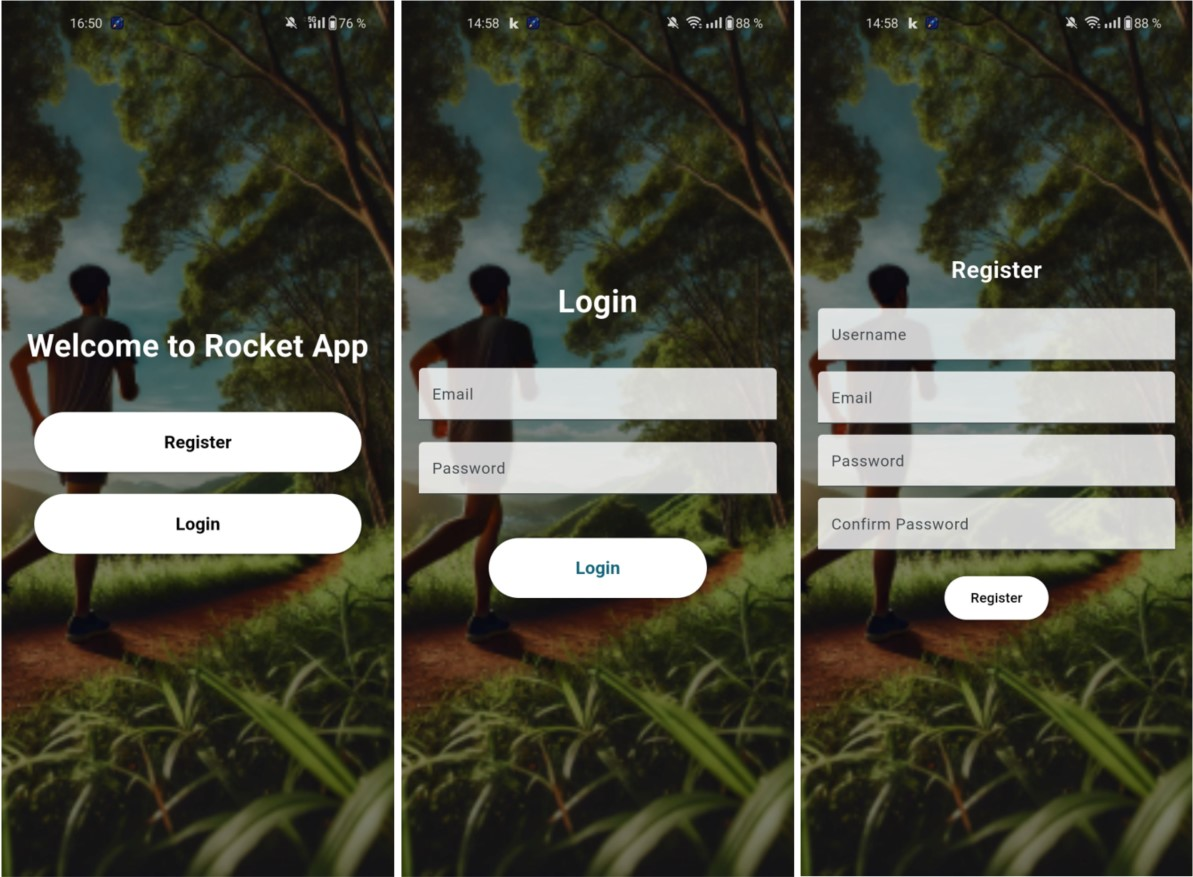
\includegraphics[width=0.7\textwidth]{images/apps/welcome-login-register-page.jpg}
    \caption{Startbildschirm der Rocket App mit Anmelde- und Registrierungsoptionen: Nutzer können sich mit E-Mail und Passwort einloggen oder ein neues Konto erstellen, um mit dem Tracking zu beginnen.}
    \label{fig:validation-workflow}
\end{figure}

Nach dem Start der App wird der Benutzer auf die \textbf{WelcomePage} geführt, die als zentrales Einstiegstor zur Anwendung dient. Dort kann zwischen den beiden Kernaktionen \textit{Login} und \textit{Registrierung} gewählt werden. Das Hintergrundbild erzeugt dabei eine motivierende visuelle Atmosphäre. Die Buttons führen jeweils zu den entsprechenden Seiten.

\paragraph{Navigation und Aufbau}
Die Navigation erfolgt über den \texttt{Navigator}-Stack von Flutter. Die Buttons sind als \texttt{ElevatedButton} umgesetzt und führen beim Tippen zur jeweiligen Seite:

\begin{lstlisting}[language=Dart, caption=Navigation zu Register- oder Login-Seite]
Navigator.push(
  context,
  MaterialPageRoute(builder: (context) => RegisterPage()),
);
\end{lstlisting}

\paragraph{Registrierungsseite}
Die \textbf{RegisterPage} enthält ein validiertes Formular mit Feldern für Benutzername, E-Mail, Passwort und Passwortbestätigung. Das Formular wird durch ein \texttt{GlobalKey<FormState>} gesteuert. Die Validierung stellt sicher, dass z.\,B. die E-Mail-Adresse korrekt formatiert ist und die Passwörter übereinstimmen.

Bei erfolgreicher Validierung wird die Registrierungsanfrage über eine asynchrone Methode an das Backend gesendet:

\begin{lstlisting}[language=Dart, caption=Registrierungsfunktion mit Backend-Aufruf]
final registerResponse = await RegisterApi.register(
  _emailController.text,
  _usernameController.text,
  _passwordController.text,
);
\end{lstlisting}

Nach erfolgreicher Registrierung wird der Nutzer automatisch zur Login-Seite weitergeleitet. Fehler, wie doppelte Benutzer oder ungültige Daten, werden über eine Snackbar angezeigt.

\paragraph{Loginseite}
Die \textbf{LoginPage} erlaubt registrierten Nutzern die Authentifizierung mittels E-Mail und Passwort. Auch hier wird ein \texttt{Form}-Widget verwendet, um Eingabefelder zu validieren. Im Erfolgsfall wird das JWT des Nutzers über die Login-API bezogen und sicher mit \texttt{flutter\_secure\_storage} gespeichert:

\begin{lstlisting}[language=Dart, caption=Speichern des JWT nach Login]
await _storage.write(key: 'jwt_token', value: loginResponse.token);
\end{lstlisting}

Da die App mit einem Foreground-Service zur Hintergrundsynchronisation arbeitet, wird das Token außerdem über \texttt{FlutterForegroundTask.sendDataToTask} an den Hintergrundprozess übergeben.

\begin{lstlisting}[language=Dart, caption=Token an Hintergrundprozess senden]
FlutterForegroundTask.sendDataToTask({'jwt_token': loginResponse.token});
\end{lstlisting}

Im Anschluss erfolgt die Weiterleitung auf die Hauptnavigation der App:

\begin{lstlisting}[language=Dart, caption=Navigation zum App-Hauptmenü]
Navigator.pushReplacement(
  context,
  MaterialPageRoute(builder: (context) => AppNavigator(title: 'Rocket App')),
);
\end{lstlisting}

\paragraph{Fehlermeldungen}
Bei Eingabefehlern oder Backend-Fehlern werden visuelle Rückmeldungen gegeben – entweder direkt im Formular oder per Snackbar. So wird sichergestellt, dass der Benutzer bei jedem Schritt eine klare Rückmeldung erhält.

\paragraph{Zusammenfassung}
Die Einstiegspunkte der App sind klar strukturiert und nutzen bewährte Flutter-Pattern für Navigation, Formularverarbeitung und Zustandshandhabung. Das Zusammenspiel aus UI, Validierung und API-Kommunikation sorgt für eine nahtlose User Experience bereits beim ersten Kontakt mit der App.

\subsection{Startseite}

\begin{figure}[H]
    \centering
    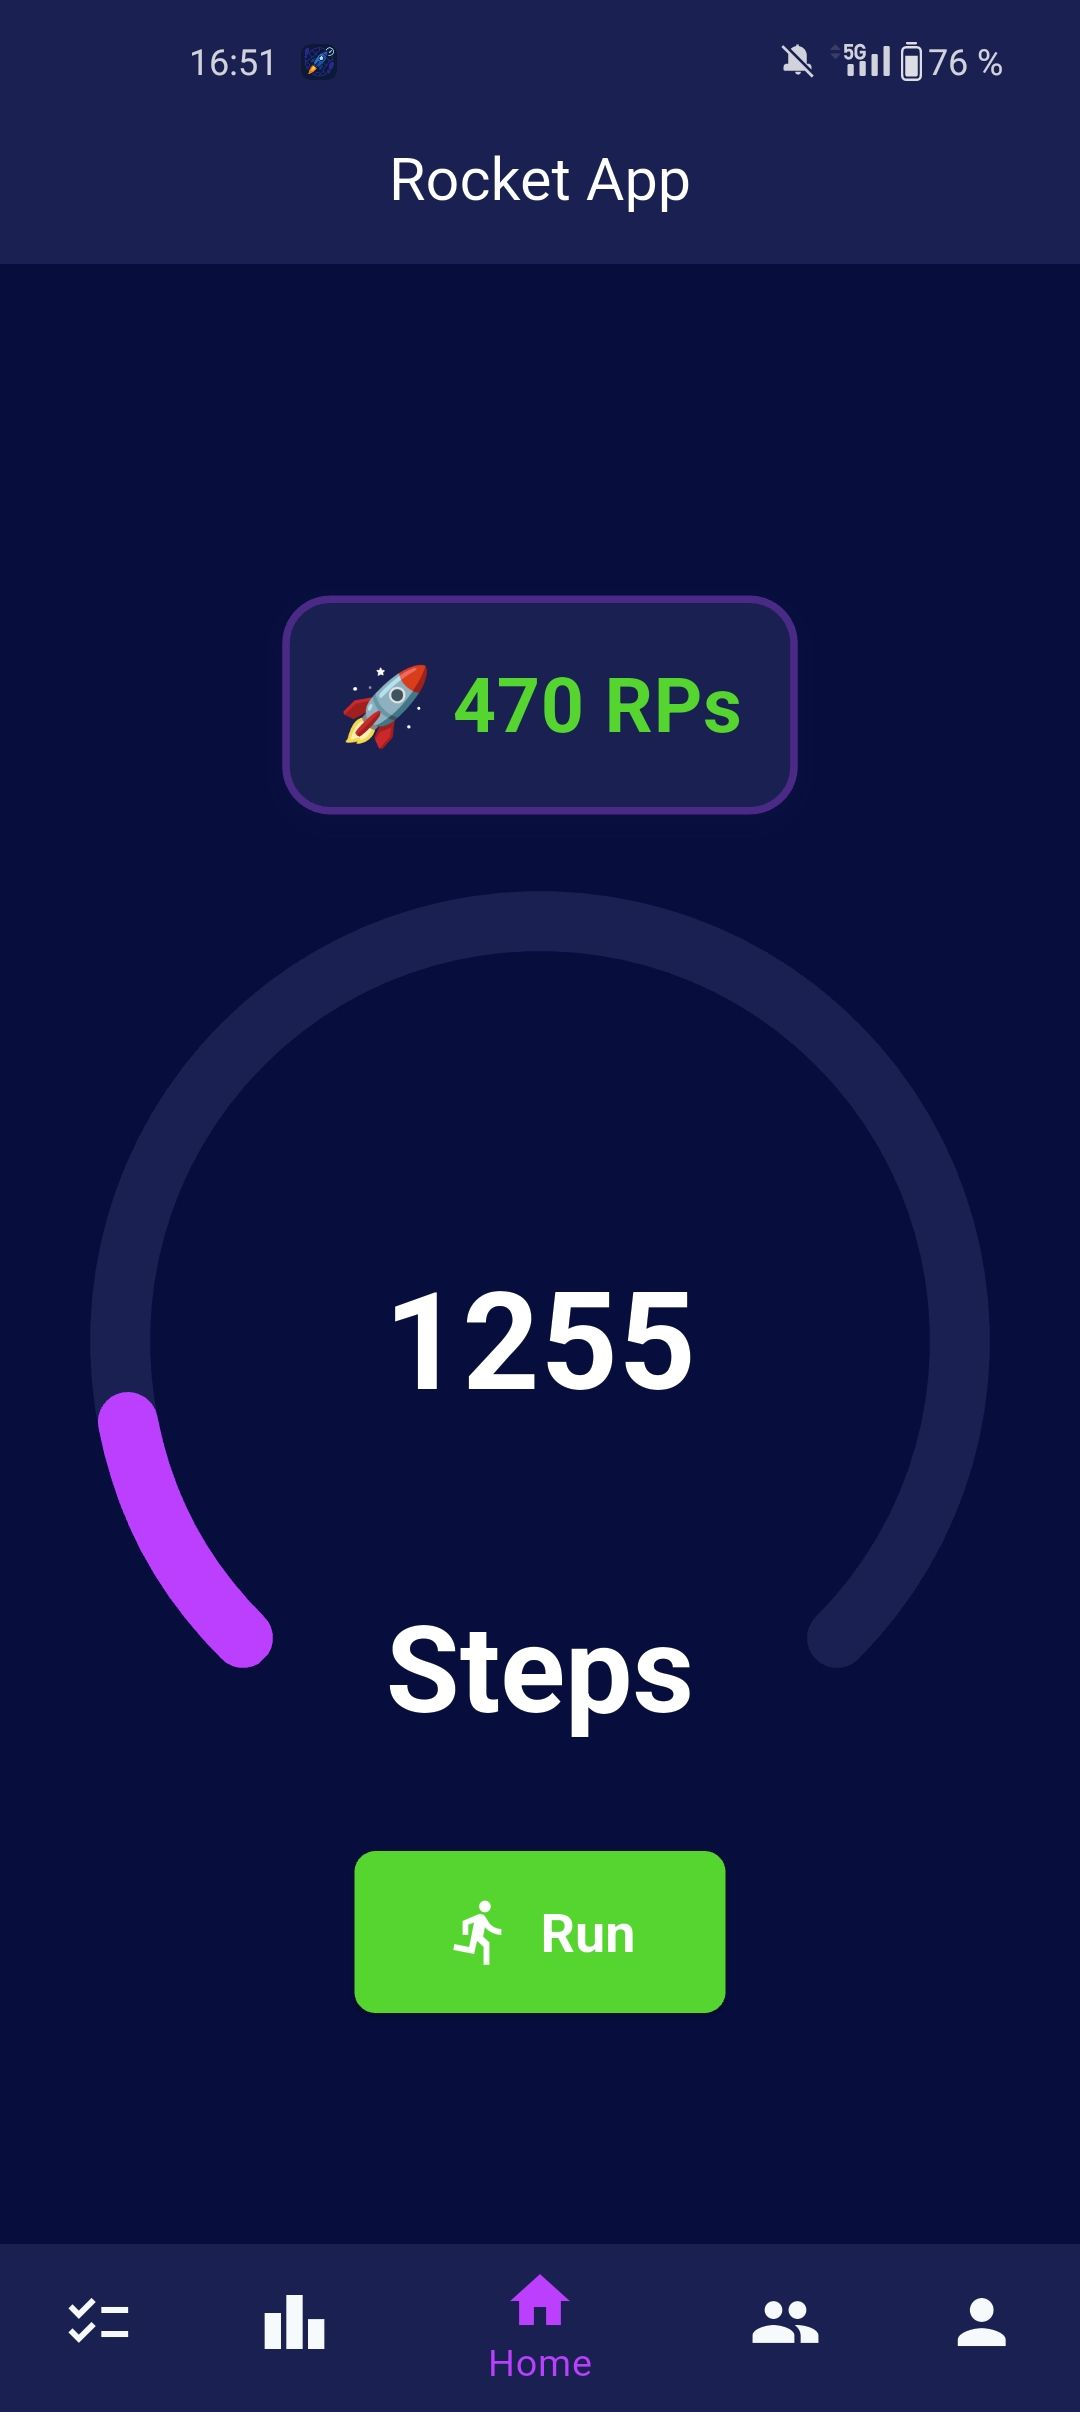
\includegraphics[width=0.25\textwidth]{images/apps/start-page.jpg}
    \caption{Startseite der Rocket App mit aktueller Schrittanzahl, verdienten Rocket Points (RPs) und „Run“-Button zum Aufrufen der Tracking-Seite.}
    \label{fig:validation-workflow}
\end{figure}

Die zentrale Startansicht der App ist die \textbf{RunPage}, die dem Nutzer eine Übersicht über seine täglichen Schritte, das aktuelle Schrittziel sowie die gesammelten Rocket Points (RPs) bietet. Über den Button \textit{Run} wird man direkt auf die Tracking-Seite weitergeleitet.

\paragraph{Datenanbindung}
Die RunPage lädt beim Start die Benutzerdaten über zwei asynchrone API-Aufrufe:
\begin{itemize}
    \item \texttt{RocketPointsApi.fetchRocketPoints(jwt)} holt die aktuellen RPs.
    \item \texttt{SettingsApi.getSettings(jwt)} liefert das individuell gesetzte Schrittziel.
\end{itemize}

Die Werte werden anschließend im State gespeichert:
\begin{lstlisting}[language=Dart, caption=Speichern von RP und Schrittziel]
setState(() {
  rocketPoints = response.rocketPoints;
  dailyGoal = settings.stepGoal;
});
\end{lstlisting}

\paragraph{Schrittfortschritt}
Die Komponente \texttt{StepCounterWidget} visualisiert den Fortschritt mit einem benutzerdefinierten Circular Painter. Die aktuelle Schrittanzahl wird dabei durch einen Foreground-Task regelmäßig aktualisiert. Der Fortschrittswert ergibt sich aus:

\[
\text{progress} = \frac{\text{currentSteps}}{\text{dailyGoal}}
\]

\begin{lstlisting}[language=Dart, caption=Progressberechnung im StepCounterWidget]
double progress = currentSteps / dailyGoal;
\end{lstlisting}

\paragraph{Rocket Points Anzeige}
Die gesammelten Rocket Points werden in einer auffälligen Karte mit Raketen-Emoji angezeigt. Diese Anzeige reagiert dynamisch auf Lade- und Fehlerzustände:

\begin{lstlisting}[language=Dart]
rocketPoints != null 
  ? '$rocketPoints RPs' 
  : '... RPs'
\end{lstlisting}

\paragraph{Navigation über BottomNavigationBar}
Die gesamte App wird über eine eigene Navigationskomponente namens \texttt{CustomMenuBar} gesteuert. Diese ist als \texttt{BottomNavigationBar} mit fünf Einträgen aufgebaut:

\begin{itemize}
    \item Challenges
    \item Leaderboard
    \item Home (zentral hervorgehoben)
    \item Friends
    \item Profile
\end{itemize}

Der Startindex der Navigation ist standardmäßig auf \texttt{2} gesetzt, womit beim App-Start automatisch die RunPage (Home) angezeigt wird.

\begin{lstlisting}[language=Dart, caption=Initiale Seitenauswahl im AppNavigator]
const AppNavigator({
  required this.title,
  this.initialIndex = 2, // Home
});
\end{lstlisting}

\paragraph{Tracking starten}
Durch Betätigen des zentralen \textit{Run}-Buttons wird die Tracking-Seite aufgerufen. Die Navigation erfolgt über einen \texttt{MaterialPageRoute}:

\begin{lstlisting}[language=Dart, caption=Navigation zur Tracking-Seite]
Navigator.push(
  context,
  MaterialPageRoute(builder: (context) => TrackingPage(title: 'Tracking')),
);
\end{lstlisting}

\paragraph{Zusammenfassung}
Die Startseite dient als tägliches Dashboard für Nutzeraktivitäten. Durch Kombination aus API-Anbindung, Live-Schrittzählung und einfacher Bedienung bildet sie den funktionalen Mittelpunkt der Rocket App.

\subsection{Runs}

\begin{figure}[H]
    \centering
    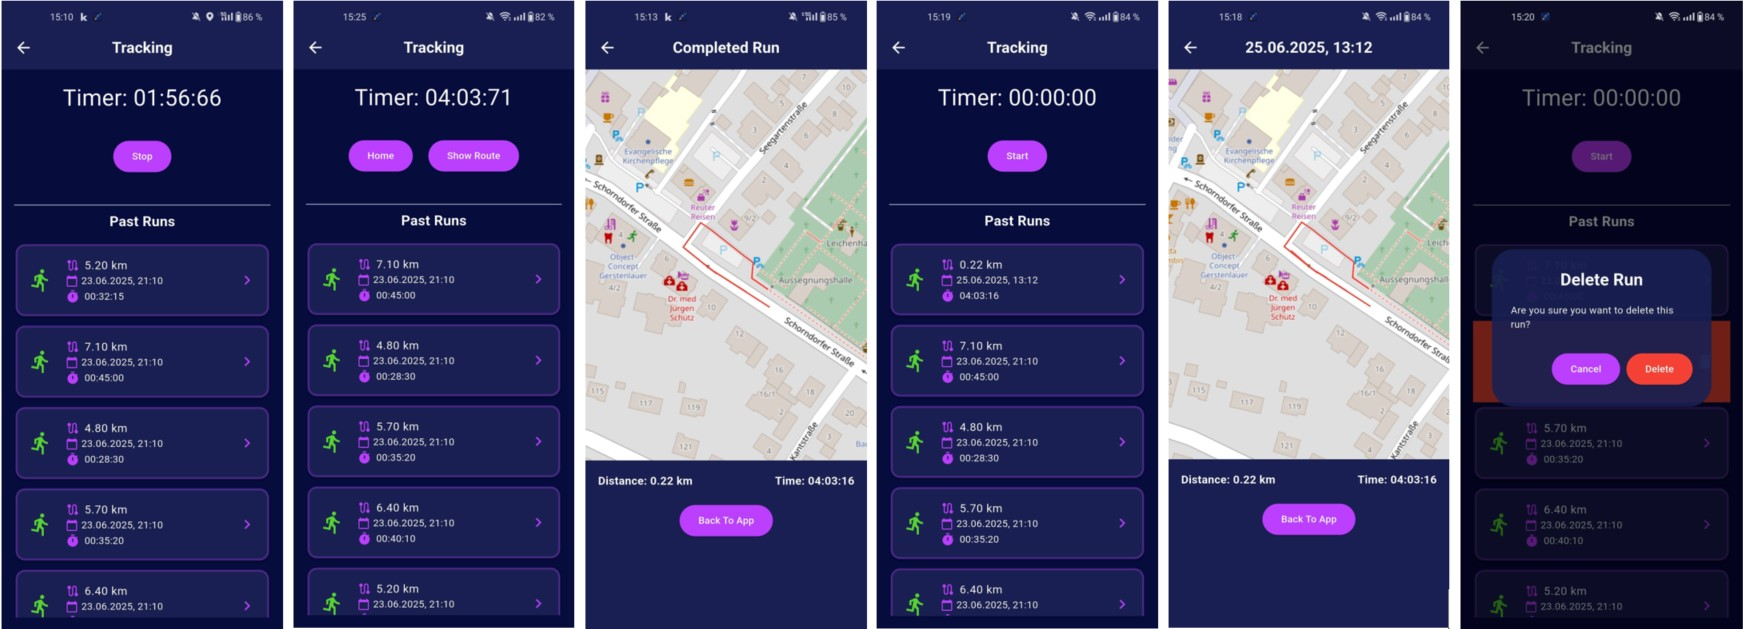
\includegraphics[width=1\textwidth]{images/apps/run-pages.jpg}
    \caption{Tracking-Bereich der Rocket App: Übersicht über vergangene Läufe mit Distanz, Zeit und Karte der Laufroute; inklusive Timer- und Tracking-Funktion, Routendarstellung und Option zum Löschen einzelner Einträge.}
    \label{fig:validation-workflow}
\end{figure}

In unserer App wird die Lauf-Route eines Nutzers kontinuierlich mithilfe von GPS-Daten erfasst. Diese Positionsdaten werden als \textit{GeoPoints} gespeichert, um später die gesamte Laufstrecke rekonstruieren und visualisieren zu können.

\subsubsection{Verwendung von OpenStreetMap}

Für die Darstellung der Routen auf der Karte setzen wir die Open-Source-Kartenplattform \textit{OpenStreetMap} (OSM)\cite{openstreetmap} ein. Die Flutter-Bibliothek \texttt{flutter\_osm\_plugin}\cite{flutter_osm_plugin} ermöglicht die nahtlose Integration der OSM-Karten in die App und bietet umfangreiche Funktionen, wie z.B. das Zeichnen von Wegen, die Anzeige von Markern und Nutzerpositionen.

OSM bietet den Vorteil, dass die Kartendaten frei verfügbar und anpassbar sind. So können wir die Laufstrecke direkt auf der Karte abbilden, indem wir die gesammelten Geo-Koordinaten als Pfad über die Karte legen.

\subsubsection{Erfassung und Speicherung der GPS-Daten}

Während eines Laufs werden fortlaufend die aktuellen GPS-Koordinaten des Nutzers abgefragt. Diese Koordinaten werden in einer Liste von \texttt{GeoPoint} Objekten gesammelt, die jeweils die \texttt{latitude} und \texttt{longitude} enthalten.

\begin{lstlisting}[language=Dart, caption=Hinzufügen eines GeoPoints zur Route]
_geoPoints.add(GeoPoint(
  latitude: position.latitude,
  longitude: position.longitude,
));
\end{lstlisting}

Diese Liste bildet die gesamte Laufstrecke ab. Neben den Geo-Koordinaten wird die verstrichene Zeit mit einem Timer gemessen und später zusammen mit der Route gespeichert.

\subsubsection{Senden der Route an das Backend}

Um die Laufdaten dauerhaft zu speichern, werden die Geo-Punkte in ein standardisiertes Format, den sogenannten \texttt{LINESTRING}, umgewandelt. Dieses Format wird häufig in geografischen Informationssystemen (GIS) verwendet, um Linien oder Wege zu repräsentieren.

\begin{lstlisting}[language=Dart, caption=Erzeugen eines LINESTRINGs]
String lineString = 'LINESTRING(' +
  _geoPoints.map((p) => '${p.longitude} ${p.latitude}').join(', ') +
  ')';
\end{lstlisting}

Die Umwandlung ist notwendig, damit das Backend die Route als eine durchgehende Linie interpretieren kann. Anschließend wird der \texttt{LINESTRING} zusammen mit der Laufzeit an die API gesendet:

\begin{lstlisting}[language=Dart, caption=Senden der Laufdaten ans Backend]
await TrackingApi.addRun(jwt, lineString, duration, distance);
\end{lstlisting}

\subsubsection{Darstellung der Route in der App}

Zur Visualisierung der gespeicherten Laufstrecken wird die Route vom Backend geladen und als Liste von GeoPoints in der App dargestellt. Über die OpenStreetMap-Karte wird dann die Strecke mit der Funktion \texttt{drawRoad} gezeichnet.

Dabei werden die einzelnen Segmente der Route als Fußwege (RoadType.foot) mit einer roten Linie hervorgehoben:

\begin{lstlisting}[language=Dart, caption=Zeichnen der Route auf der Karte]
for (int i = 0; i < _routePoints.length - 1; i++) {
  await _mapController.drawRoad(
    _routePoints[i],
    _routePoints[i + 1],
    roadType: RoadType.foot,
    roadOption: RoadOption(
      roadColor: Colors.red,
      roadWidth: 8,
    ),
  );
}
\end{lstlisting}

Diese Visualisierung ermöglicht dem Nutzer, die genaue Strecke seines Laufs nachvollziehen zu können. Zusätzlich werden wichtige Informationen wie Gesamtdistanz und Laufzeit übersichtlich angezeigt.

\subsubsection{Berechnung der Gesamtdistanz}

Die Gesamtdistanz wird aus den GeoPoints berechnet, indem für jedes aufeinanderfolgende Punktpaar die Entfernung mithilfe der Haversine-Formel bestimmt wird. Diese Formel berechnet die kürzeste Entfernung über die Erdoberfläche zwischen zwei Koordinaten.

\begin{lstlisting}[language=Dart, caption=Berechnung der Entfernung zweier GeoPoints]
double _calculateDistanceBetween(GeoPoint a, GeoPoint b) {
  const double R = 6371; // Erdradius in Kilometern
  double dLat = _deg2rad(b.latitude - a.latitude);
  double dLon = _deg2rad(b.longitude - a.longitude);
  double lat1 = _deg2rad(a.latitude);
  double lat2 = _deg2rad(b.latitude);

  double hav = sin(dLat / 2) * sin(dLat / 2) +
      sin(dLon / 2) * sin(dLon / 2) * cos(lat1) * cos(lat2);
  double c = 2 * atan2(sqrt(hav), sqrt(1 - hav));
  return R * c;
}
\end{lstlisting}

Die Summe aller Teilstrecken ergibt die Gesamtstrecke des Laufs.

\subsubsection{Verwaltung von Läufen}

Alle gespeicherten Läufe werden unterhalb des Timers in einer Liste dargestellt. Jeder Eintrag zeigt:

\begin{itemize}
  \item die zurückgelegte Distanz,
  \item das Datum und die Uhrzeit des Laufs,
  \item sowie die Laufdauer.
\end{itemize}

\paragraph{Lauf starten und stoppen}

Ein Lauf kann durch Tippen auf die \texttt{Start}-Schaltfläche begonnen werden. Dabei wird ein \texttt{Stopwatch} aktiviert, um die Zeit zu messen, und über die \texttt{Geolocator}-Bibliothek werden kontinuierlich GPS-Daten aufgezeichnet. Während des Laufens wird die Zeit in Echtzeit oben im Interface angezeigt.

Nach dem Laufen kann der Nutzer den Lauf durch Tippen auf \texttt{Stop} beenden. Anschließend erscheint eine neue Auswahl: Die Route kann angezeigt (\texttt{Show Route}) oder zur Startseite zurückgekehrt werden (\texttt{Home}).

\begin{lstlisting}[language=Dart, caption=Starten des Trackings]
setState(() {
  _isTracking = true;
  _geoPoints.clear();
  _stopwatch.reset();
  _stopwatch.start();
});
\end{lstlisting}

\begin{lstlisting}[language=Dart, caption=Stoppen des Trackings und Speichern]
_stopwatch.stop();
_positionStream?.cancel();
await TrackingApi.addRun(jwt, lineString, duration, distance);
\end{lstlisting}

\paragraph{Einsehen eines gespeicherten Laufs}

Durch Tippen auf einen Listeneintrag in der Historie wird die zugehörige Laufroute auf einer Karte visualisiert. Hierzu wird die gespeicherte \texttt{LINESTRING}-Route zurück in \texttt{GeoPoints} konvertiert und mit der Funktion \texttt{drawRoad} auf der OpenStreetMap-Karte gezeichnet. Zusätzlich werden Distanz und Dauer erneut eingeblendet.

\begin{lstlisting}[language=Dart, caption=Navigation zur Detailansicht einer Route]
Navigator.push(
  context,
  MaterialPageRoute(
    builder: (context) => RoutePage(
      title: _formatDate(run.createdAt),
      routePoints: parseLineString(run.route),
      elapsedTime: run.duration,
    ),
  ),
);
\end{lstlisting}

\paragraph{Löschen eines Laufs}

Durch ein Wischen (Swipe) eines Lauf-Eintrags nach links wird die Option eingeblendet, den Lauf zu löschen. Bevor die Daten endgültig entfernt werden, erscheint ein Dialog zur Bestätigung der Aktion. Dies verhindert versehentliches Löschen und erhöht die Nutzerfreundlichkeit.

\begin{lstlisting}[language=Dart, caption=Löschbestätigung per Dialog]
confirmDismiss: (direction) async {
  return await showDialog(
    context: context,
    builder: (context) => AlertDialog(
      title: Text('Delete Run'),
      content: Text('Are you sure you want to delete this run?'),
      actions: [
        ElevatedButton(onPressed: () => Navigator.of(context).pop(false), child: Text('Cancel')),
        ElevatedButton(onPressed: () => Navigator.of(context).pop(true), child: Text('Delete')),
      ],
    ),
  );
},
\end{lstlisting}

\begin{lstlisting}[language=Dart, caption=Entfernen des Laufs aus der Datenbank]
await TrackingApi.deleteRun(jwt, run.id);
\end{lstlisting}

Diese Funktionen bilden zusammen eine vollständige Tracking-Suite, mit der Nutzer ihre Aktivitäten genau aufzeichnen, verwalten und visualisieren können.

\subsection{Freundesliste}

\begin{figure}[H]
    \centering
    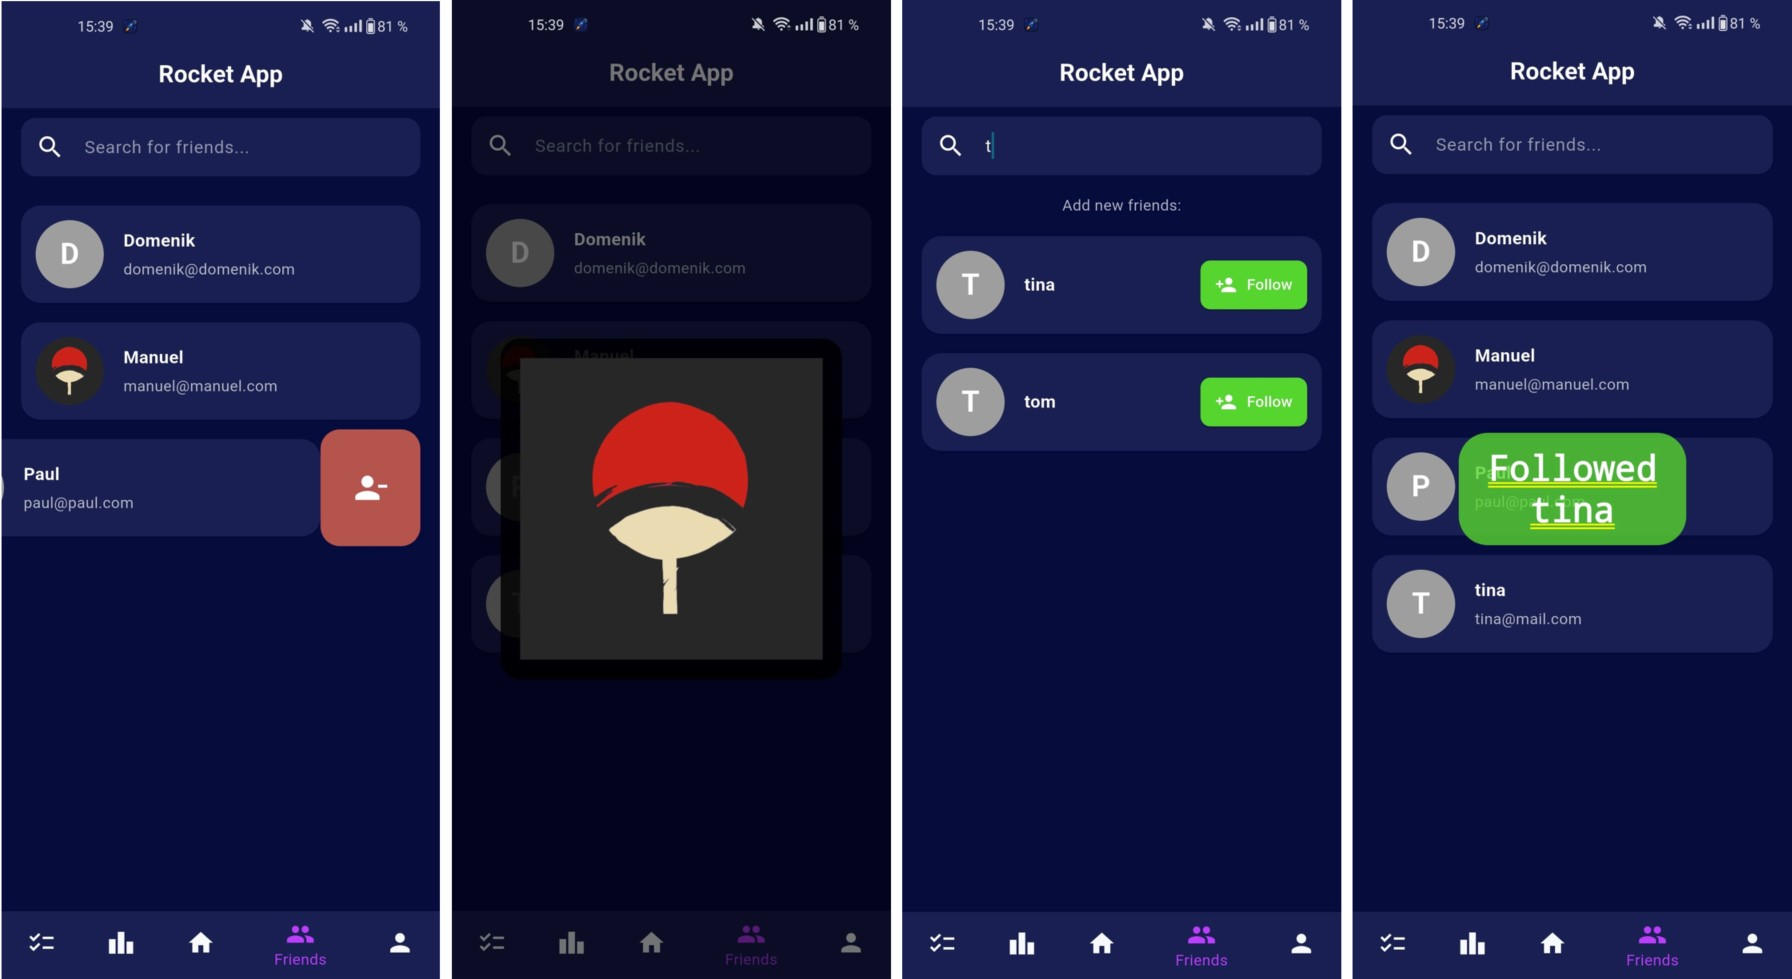
\includegraphics[width=0.85\textwidth]{images/apps/friendlist-pages.jpg}
    \caption{Freundesliste der Rocket App: Nutzer können nach Freunden suchen, Kontakte hinzufügen oder entfernen sowie deren Mailadresse einsehen.}
    \label{fig:validation-workflow}
\end{figure}


Die Freundesliste ist ein zentraler Bestandteil der sozialen Interaktion innerhalb der Rocket App. Sie erlaubt das Verwalten bestehender Kontakte sowie das gezielte Suchen und Hinzufügen neuer Nutzer.
Sie ermöglicht es Nutzer:innen somit, mit anderen Personen in Kontakt zu treten. Die Funktionalität wird durch serverseitige API-Abfragen in Kombination mit lokalen Filtern ermöglicht.

\paragraph{Suchfunktion und Nutzerliste}
Oberhalb der Ansicht befindet sich eine Suchleiste, mit der gezielt nach Nutzern anhand ihres Usernamens gesucht werden kann. Die Eingabe filtert dynamisch sowohl:
\begin{itemize}
    \item bereits gefolgte Freunde (links in der Abbildung) und
    \item nicht gefolgte Nutzer, die mit einem ``\texttt{Follow}''-Button angezeigt werden (dritte Ansicht).
\end{itemize}

Bei jeder Eingabe (über \texttt{onChanged}) wird der Zustand \texttt{\_searchQuery} aktualisiert. Die Liste der bereits gefolgten Freunde sowie möglicher neuer Kontakte wird in der \texttt{build()}-Methode auf Basis dieses Werts dynamisch gefiltert. Die Filterung funktioniert über eine \textbf{Substring-Suche}: Der eingegebene Suchtext wird mit jedem Benutzernamen (kleinbuchstaben-normalisiert) verglichen. Enthält der Benutzername den Suchtext, wird das Element angezeigt: 

\begin{lstlisting}[language=Dart, caption=Filter-Logik für Freundesliste und Suchergebnisse]
final filteredFriends = friends.where((f) =>
  _searchQuery.isEmpty || f.username.toLowerCase().contains(_searchQuery.toLowerCase())
).toList();

final searchResults = allUsers.where((u) {
  final matchesQuery = _searchQuery.isNotEmpty &&
                       u.username.toLowerCase().contains(_searchQuery.toLowerCase());
  final notFriendYet = !friends.any((f) => f.id == u.id);
  return matchesQuery && notFriendYet;
}).toList();
\end{lstlisting}

\paragraph{Freunde entfernen per Swipe-Geste}
Bereits gefolgte Kontakte lassen sich per Swipe-Geste (nach links) über das \texttt{flutter\_slidable}-Paket entfernen. Es erscheint eine Schaltfläche zum Entfernen des Freundes (\texttt{Icons.person\_remove}). Ein Tap löst einen API-Aufruf aus, um den Kontakt serverseitig zu löschen. Danach wird die Freundesliste neu geladen.



\begin{lstlisting}[language=Dart, caption=Unfollow eines Freundes per Slidable]
await FriendsApi.deleteFriend(jwt, friend.username);
final freshFriends = await FriendsApi.getAllFriends(jwt);
setState(() {
  friends = freshFriends;
});
\end{lstlisting}

\paragraph{Bestehende Freunde anzeigen und entfernen}
Bereits gefolgte Nutzer:innen werden als Karten in einer Liste angezeigt. Diese Karten enthalten:
\begin{itemize}
    \item den Nutzernamen
    \item die E-Mail-Adresse
    \item ein Profilbild (oder Initiale, falls kein Bild vorhanden ist)
\end{itemize}
Sowohl für bestehende als auch neue Kontakte wird das Profilbild angezeigt – sofern verfügbar. Fehlt ein Bild, wird stattdessen der erste Buchstabe des Nutzernamens dargestellt. Bei Klick auf ein Profilbild wird es in einer vergrößerten Ansicht angezeigt.

\begin{lstlisting}[language=Dart, caption=Profilbildanzeige und Zoom-Dialog]
GestureDetector(
  onTap: () => _showImageDialog(friend.imageData!),
  child: CircleAvatar(
    backgroundImage: MemoryImage(friend.imageData!),
  ),
);
\end{lstlisting}
\paragraph{Neue Freunde suchen und hinzufügen}
Wird ein Benutzername eingegeben, der zu Nutzer:innen passt, die noch nicht gefolgt werden, erscheinen diese unter dem Abschnitt \textit{Add new friends}. Jede Karte zeigt Username und Bild sowie einen grünen ``Follow''-Button.

Bei Betätigen dieses Buttons:
\begin{enumerate}
    \item wird ein \texttt{POST}-Request an die API \texttt{/api/v1/protected/friends/add} gesendet,
    \item die Freundesliste und Userliste wird lokal aktualisiert (\texttt{setState}),
    \item die Eingabe wird geleert,
    \item und ein \textbf{Overlay-Popup} mit dem Text \texttt{Followed <name>} erscheint für 2 Sekunden.
\end{enumerate}

\begin{lstlisting}[language=Dart, caption=Freund hinzufügen und Overlay anzeigen]
await FriendsApi.addFriend(jwt, user.username);
_showFollowOverlay(user.username);
\end{lstlisting}

\begin{lstlisting}[language=Dart, caption=Overlay-Feedback nach erfolgreichem Hinzufügen]
OverlayEntry(
  builder: (context) => Center(
    child: Container(
      child: Text('Followed\n$name'),
    ),
  ),
);
\end{lstlisting}

\paragraph{Asynchrone Datenbindung und Sicherheit}
Die gesamte Seite ist ebenfalls durch einen sicheren Authentifizierungstoken (JWT) abgesichert, der lokal über \texttt{flutter\_secure\_storage} ausgelesen wird. Alle Serverzugriffe (z.B. \texttt{getAllFriends}, \texttt{addFriend}, \texttt{deleteFriend}) verwenden diesen Token im Header.

\paragraph{Design und Farben}
Alle Einträge (Friend-Cards) sind optisch abgesetzt, farblich abwechselnd hinterlegt (dunkelblau und violett) und enthalten:
\begin{itemize}
    \item Profilbild bzw. Initiale
    \item Nutzername
    \item E-Mail-Adresse
\end{itemize}

Durch die Kombination aus direkter Interaktion, visuellem Feedback und API-Anbindung stellt die Freundesliste ein intuitives und funktionales Element der App dar, das soziale Vernetzung aktiv unterstützt. Durch die sichere, asynchrone Datenbindung und die enge Verzahnung mit dem Server-Backend wird eine stets aktuelle und konsistente Darstellung der sozialen Kontakte innerhalb der App gewährleistet.

\subsection{Challenges}

\begin{figure}[H]
    \centering
    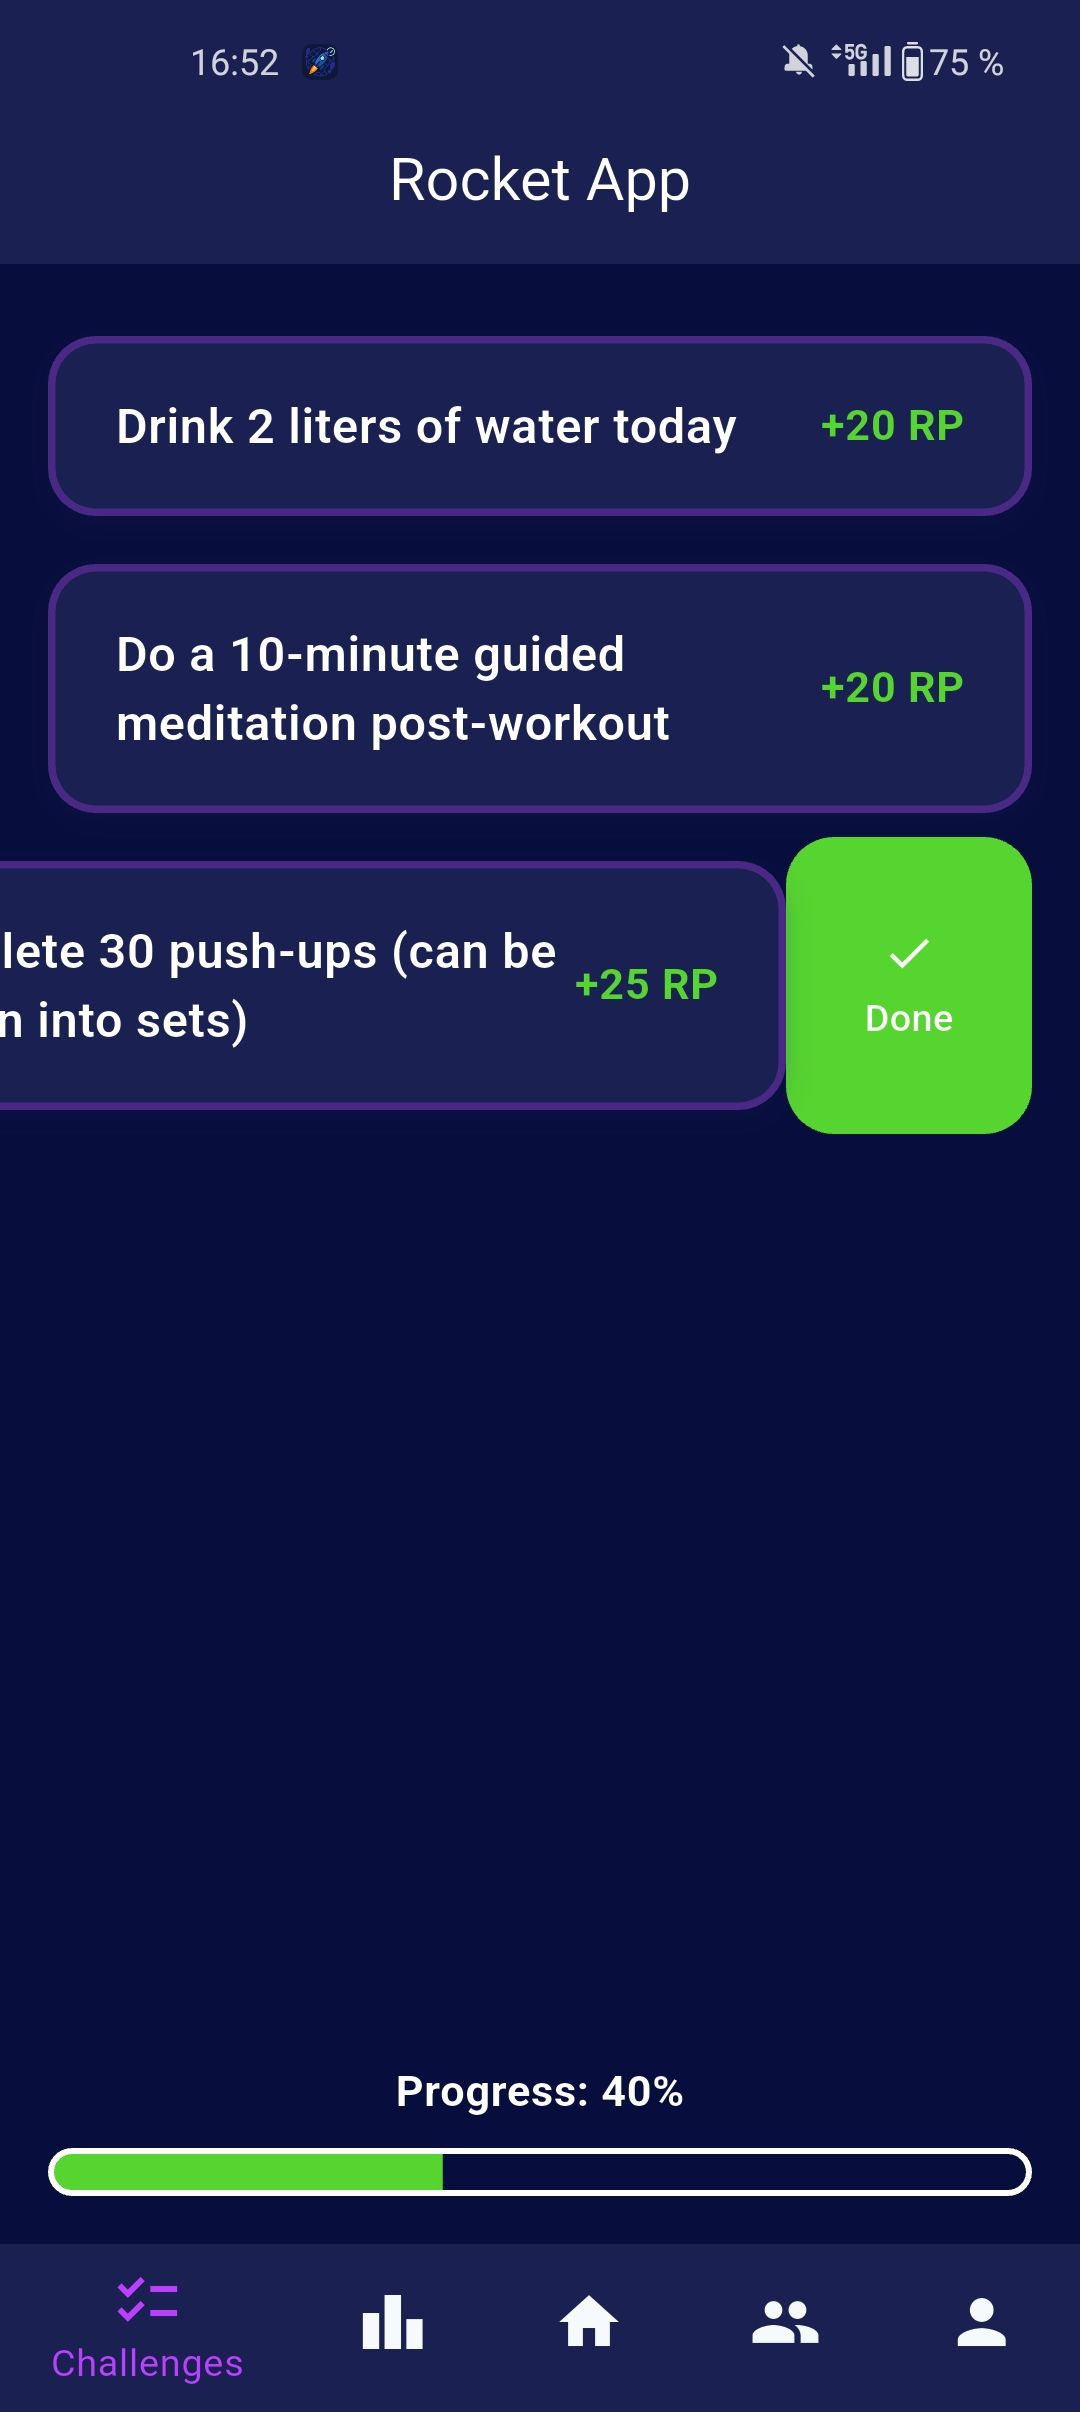
\includegraphics[width=0.25\textwidth]{images/apps/challenge-page.jpg}
    \caption{Challenges-Ansicht der Rocket App: Nutzer können tägliche Aufgaben wie Trinken, Meditation oder Push-ups absolvieren und dafür Rocket Points sammeln – inklusive Fortschrittsanzeige in Prozent.}
    \label{fig:validation-workflow}
\end{figure}

Die Challenge-Seite zeigt eine Auswahl an täglichen Aufgaben, die Nutzer:innen zur Förderung eines gesunden Lebensstils absolvieren können. Jede absolvierte Aufgabe wird mit sogenannten \textbf{Rocket Points (RP)} belohnt. Die Seite bietet dabei sowohl eine klare Übersicht über aktuelle Challenges als auch eine visuelle Rückmeldung über Fortschritt und Erfolge.

\paragraph{Laden der Herausforderungen}
Beim Öffnen der Seite werden zunächst alle aktuellen täglichen Challenges per API geladen:

\begin{lstlisting}[language=Dart, caption=Laden der Tages-Challenges vom Server]
final challenges = await ChallengesApi.fetchChallenges(jwt);
setState(() {
  _challenges = challenges;
});
\end{lstlisting}

Zusätzlich wird der aktuelle Fortschritt abgerufen – also wie viele Challenges bereits erledigt wurden und wie viele insgesamt verfügbar sind:

\begin{lstlisting}[language=Dart, caption=Abfrage des Challenge-Fortschritts]
final progress = await ChallengesApi.fetchChallengeProgress(jwt);
_completedChallenges = progress.completed;
_totalChallenges = progress.total == 0 ? 1 : progress.total;
\end{lstlisting}

\paragraph{Darstellung der Challenges}
Jede Challenge wird als visuell abgesetzte Karte mit zwei Informationen angezeigt:
\begin{itemize}
    \item \textbf{Beschreibung der Aufgabe} (z.\,B. ``Drink 2 liters of water today'')
    \item \textbf{Belohnung in Rocket Points} (z.\,B. ``+20 RP'')
\end{itemize}

Die Karten besitzen ein modernes Design mit weichem Schatten, abgerundeten Ecken und einem farblich abgesetzten Rand. Die Gestaltung ist vollständig dynamisch und anpassbar über zentrale Farbkonsstanten.

\paragraph{Markieren als erledigt (Swipe to complete)}
Eine Challenge kann als \textbf{„erledigt“} markiert werden, indem die Karte entweder nach links oder rechts gewischt wird – realisiert mit \texttt{flutter\_slidable}. Dabei wird folgende Logik ausgeführt:

\begin{enumerate}
    \item Die Challenge wird aus der Liste entfernt
    \item Eine API-Anfrage markiert sie als erledigt
    \item Die Fortschrittsanzeige wird aktualisiert
    \item Eine visuelle Animation mit den gewonnenen Punkten erscheint
\end{enumerate}

\begin{lstlisting}[language=Dart, caption=Challenge als erledigt markieren]
await ChallengesApi.markAsDone(jwt, challenge.id, challenge.points);
setState(() {
  _challenges.remove(challenge);
});
\end{lstlisting}

\paragraph{Visuelles Feedback: RP-Overlay}
Wird eine Challenge abgeschlossen, erscheint ein animiertes Overlay, das die erhaltenen Punkte anzeigt. Es wird zentral im Bildschirm eingeblendet, bewegt sich nach oben und verblasst anschließend. Dabei kommen Flutter-Animationen und ein \texttt{OverlayEntry} zum Einsatz:

\begin{lstlisting}[language=Dart, caption=Overlay mit Punktanzeige bei Erfolg]
OverlayEntry(
  builder: (context) => Center(
    child: Text('+25 RP', style: TextStyle(...)),
  ),
);
\end{lstlisting}

\paragraph{Fortschrittsbalken}
Am unteren Rand wird der aktuelle Fortschritt durch einen \textbf{linearen Balken} dargestellt. Die Prozentzahl basiert auf dem Verhältnis von erledigten zu allen täglichen Challenges. Sowohl der Text ``Progress: 40\%'' als auch der Balken selbst aktualisieren sich automatisch.

\begin{lstlisting}[language=Dart, caption=Berechnung des Fortschrittswertes]
double progressValue = (_completedChallenges / _totalChallenges).clamp(0.0, 1.0);
\end{lstlisting}

Der Balken nutzt eine abgerundete Rahmenstruktur mit weißem Rand und ist in leuchtendem Grün gefüllt, sobald Fortschritte erzielt werden.

\paragraph{Ziel und Motivation}
Die Challenges sind ein integraler Bestandteil der Gamification-Strategie der Rocket App. Sie dienen dazu, Alltagsaufgaben in spielerischer Form mit messbaren Fortschritten zu verknüpfen. Durch visuelle Belohnungen, Swipe-Gesten und Fortschrittsanzeige entsteht ein direkter Anreiz zur täglichen Nutzung.

\vspace{1em}
Die API-Endpunkte, die zur Realisierung dieser Seite genutzt werden, sind unter Abschnitt \texttt{/api/v1/protected/challenges} dokumentiert.

\subsection{Leaderboard}

\begin{figure}[H]
    \centering
    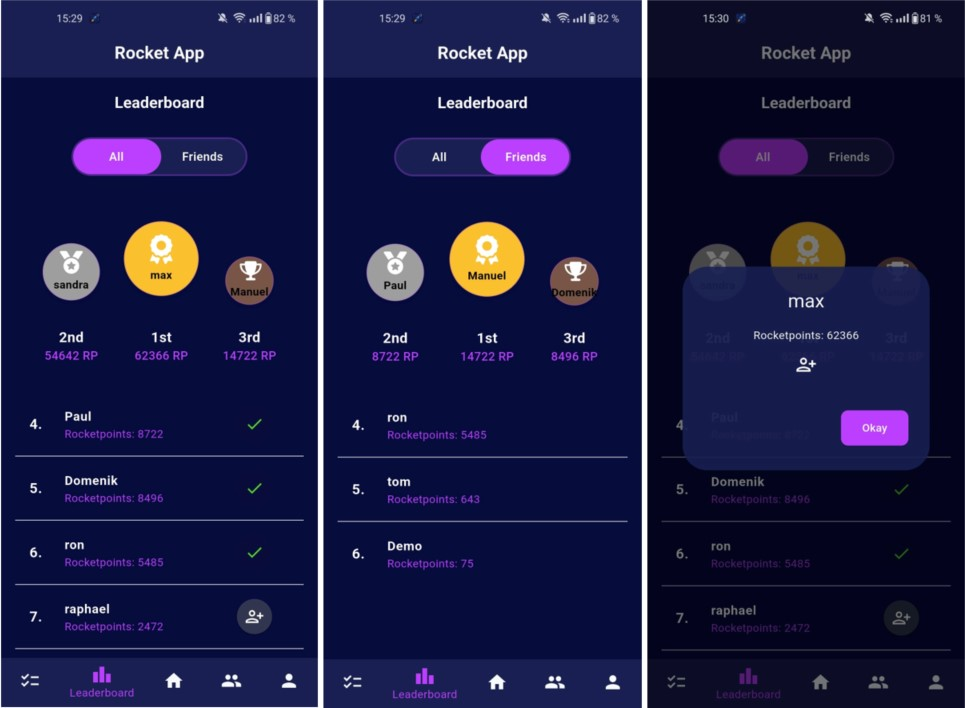
\includegraphics[width=0.7\textwidth]{images/apps/leaderboard.jpg}
    \caption{Leaderboard der Rocket App: Anzeige der globalen und freundesbezogenen Rangliste basierend auf gesammelten Rocket Points – mit Detailansicht einzelner Nutzerprofile.}
    \label{fig:validation-workflow}
\end{figure}

Die Leaderboard-Ansicht visualisiert den aktuellen Punktestand aller Nutzer:innen der Rocket App. Sie dient als soziales Vergleichselement und fördert die Motivation durch Ranglistenmechanismen. Dabei können wahlweise:
\begin{itemize}
    \item alle Nutzer:innen (\textit{All}) oder
    \item nur Freund:innen (\textit{Friends})
\end{itemize}
angezeigt werden.

\paragraph{Tab-Umschaltung (All vs. Friends)}
Die Ansicht verwendet einen animierten Umschalter zur Auswahl zwischen den zwei Modi. Die jeweils angezeigte Liste (\texttt{displayedUsers}) wird beim Umschalten aktualisiert:

\begin{lstlisting}[language=Dart, caption=Wechsel zwischen allen Nutzer:innen und Freund:innen]
void switchTab(int tabIndex) {
  setState(() {
    selectedTab = tabIndex;
    displayedUsers = tabIndex == 0 ? allUsers : friends;
  });
}
\end{lstlisting}

\paragraph{Platz 1–3: Podestanzeige}
Die drei führenden Nutzer:innen werden prominent auf einem Podium dargestellt. Jeder Platz (1.–3.) ist farblich und größenmäßig differenziert:
\begin{itemize}
    \item \textbf{Gold} für Platz 1 mit größtem Avatar
    \item \textbf{Silber} für Platz 2
    \item \textbf{Bronze} für Platz 3
\end{itemize}

Die Avatare beinhalten einen Rang-Icon (Medaille, Award, Pokal) sowie den Namen. Ein Tap auf den Avatar öffnet ein modales Dialogfenster mit weiteren Infos.

\paragraph{Detaildialog mit Freundschaftsoption}
Wird auf einen Podest-Avatar getippt, erscheint ein modaler Dialog (\texttt{AlertDialog}), der Folgendes zeigt:
\begin{itemize}
    \item Benutzername
    \item Gesamtpunktzahl
    \item Option zum Hinzufügen als Freund (sofern noch nicht befreundet)
\end{itemize}

\begin{lstlisting}[language=Dart, caption=Dialog zur Freundschaftsanfrage aus dem Podium]
IconButton(
  icon: Icon(isFriend(user) ? Icons.check : Icons.person_add_alt),
  onPressed: isFriend(user) ? null : () async {
    addFriend(user);
    Navigator.of(context).pop();
  },
);
\end{lstlisting}

\paragraph{Rangliste ab Platz 4}
Alle weiteren Nutzer:innen (ab Platz 4 oder ab Platz 1, wenn <3) werden unter dem Podium in einer scrollbaren Liste angezeigt. Jede Zeile enthält:
\begin{itemize}
    \item Rangnummer
    \item Benutzername
    \item Aktueller Punktestand
    \item Freundschaftsstatus (Icon zum Hinzufügen oder Häkchen)
\end{itemize}

Ist man bereits mit einem Nutzer befreundet, wird ein grüner Haken angezeigt. Andernfalls erscheint ein ``Add Friend''-Icon als Button.

\paragraph{Freund:innen hinzufügen aus der Rangliste}
Nutzer:innen im ``All''-Modus können direkt durch Tippen auf das Icon als Freund hinzugefügt werden. Der Button wird nach erfolgreichem API-Call deaktiviert.

\begin{lstlisting}[language=Dart, caption=Freundschaft aus der Rangliste anfragen]
ElevatedButton(
  onPressed: isFriend(user) ? null : () => addFriend(user),
  child: Icon(isFriend(user) ? Icons.check : Icons.person_add_alt),
);
\end{lstlisting}

\paragraph{Datenquelle und Aktualisierung}
Die Daten für beide Listen (``All'' und ``Friends'') werden beim Initialisieren der Seite über einen gesicherten API-Aufruf geladen. Verwendet wird ein lokal gespeicherter JWT:

\begin{lstlisting}[language=Dart, caption=Laden der Ranglisten über API]
final fetchedAllUsers = await RankingApi.fetchUserRankings(jwt);
final fetchedFriends = await RankingApi.fetchFriendRankings(jwt);
\end{lstlisting}

Die Daten bleiben so lange bestehen, bis die Seite verlassen oder manuell aktualisiert wird. Beim Hinzufügen eines neuen Freundes wird die Freundesliste ergänzt.

\paragraph{Funktion und Motivation}
Das Leaderboard steigert die Nutzerbindung durch Wettbewerb. Die visuelle Podiumsdarstellung, unmittelbare Vergleichbarkeit sowie einfache Interaktionsmöglichkeiten (z.\,B. neue Freund:innen entdecken) fördern eine nachhaltige und aktive Nutzung der App.

\vspace{1em}
Die zugehörigen Backend-Endpunkte finden sich unter \texttt{/api/v1/protected/leaderboard} und \texttt{/friends/add}.

\subsection{Profil und Einstellungen}

\begin{figure}[H]
    \centering
    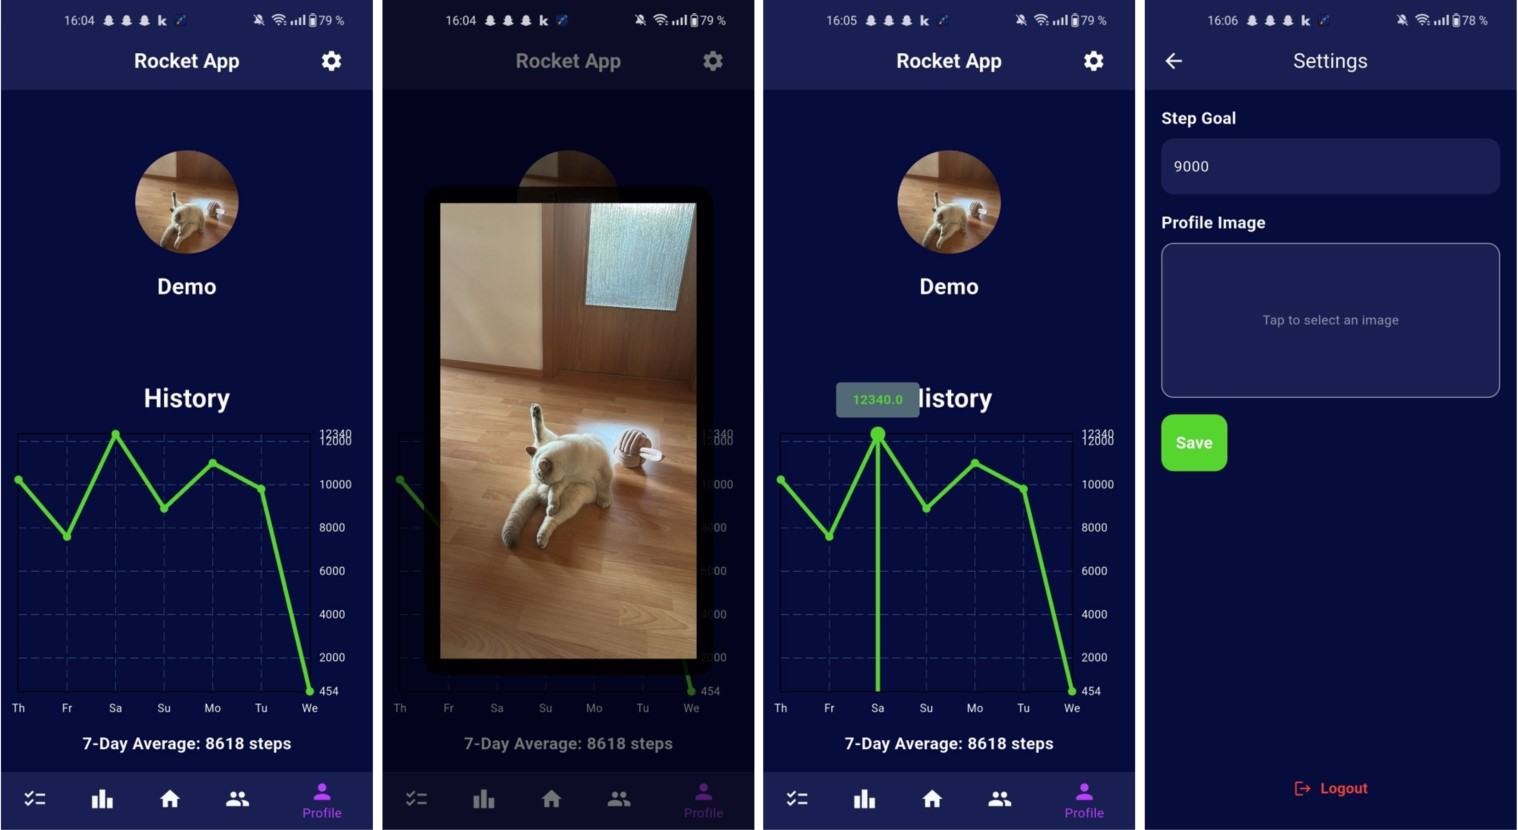
\includegraphics[width=0.9\textwidth]{images/apps/profile-settings-page.jpg}
    \caption{Profil- und Einstellungsbereich der Rocket App: Anzeige der Schritt-Historie mit 7-Tage-Durchschnitt, Möglichkeit zur Änderung des Profilbilds sowie Festlegung eines individuellen Schrittziels}
    \label{fig:validation-workflow}
\end{figure}

\subsubsection{Profilseite}

Die Profilseite kombiniert zwei Hauptkomponenten: ein Profilbild mit Nutzernamen (oben) sowie eine visuelle Darstellung der Schrittanzahl der letzten sieben Tage (unten).

\paragraph{Profilbild \& Username}
Das Profilbild wird beim Laden der Seite per API von einem Base64-codierten String in ein Bild umgewandelt und in einem runden Avatar dargestellt. Ist kein Bild vorhanden, wird stattdessen der Anfangsbuchstabe des Benutzernamens gezeigt. Beim Antippen des Bildes wird dieses in einem modalen Vollbilddialog angezeigt:

\begin{lstlisting}[language=Dart, caption=Bild als Dialog anzeigen]
GestureDetector(
  onTap: () => _showImageDialog(Uint8List.fromList(imageData)),
  child: CircleAvatar(...),
);
\end{lstlisting}

\paragraph{Schritthistorie (Line Chart)}
Darunter befindet sich ein Liniendiagramm, das die tägliche Schrittanzahl der vergangenen sieben Tage visualisiert. Die Datenpunkte werden per API geladen, wobei jeder Punkt einem Wochentag zugeordnet ist. 

Die Darstellung nutzt das Paket \texttt{fl\_chart}. Das Diagramm zeigt:
\begin{itemize}
  \item Tagesnamen auf der x-Achse
  \item Schrittanzahl auf der y-Achse (rechte Seite)
  \item Durchschnittswert als Zahl unter dem Diagramm
\end{itemize}

\begin{lstlisting}[language=Dart, caption=Diagrammkonfiguration für Schrittverlauf]
LineChartBarData(
  spots: List.generate(
    stepsData.length,
    (index) => FlSpot(index.toDouble(), stepsData[index]),
  ),
  isCurved: false,
  color: ColorConstants.greenColor,
  barWidth: 4,
);
\end{lstlisting}

Beim Antippen eines Tages erscheint oberhalb der Kurve ein Tooltip, der die genaue Schrittanzahl für diesen Tag anzeigt.

\subsubsection{Einstellungsseite}

Die Einstellungsseite bietet zwei konfigurierbare Optionen:
\begin{itemize}
  \item Tägliches Schrittziel (numerischer Wert)
  \item Profilbild (uploadbar aus Galerie)
\end{itemize}

\paragraph{Schrittziel anpassen}
Das Ziel kann frei gewählt und gespeichert werden. Eingabefehler wie ungültige Zahlen oder leere Felder werden dabei abgefangen:

\begin{lstlisting}[language=Dart, caption=Gültigkeitsprüfung Schrittziel]
if (stepGoal == null || stepGoal <= 0) {
  _errorMessage = 'Please enter a valid step goal greater than 0';
}
\end{lstlisting}

\paragraph{Profilbild ändern}
Durch Antippen des Upload-Felds öffnet sich die Bildgalerie. Nach Auswahl wird das Bild in der UI angezeigt und beim ``Save''-Klick hochgeladen:

\begin{lstlisting}[language=Dart, caption=Bild aus Galerie auswählen]
final pickedFile = await picker.pickImage(source: ImageSource.gallery);
if (pickedFile != null) {
  _selectedImage = File(pickedFile.path);
}
\end{lstlisting}

\paragraph{Daten speichern}
Nach Klick auf ``Save'' werden Schrittziel und Profilbild über zwei separate API-Aufrufe gespeichert. Bei Erfolg erscheinen Snackbar-Benachrichtigungen.

\paragraph{Logout-Funktion}
Ein ``Logout''-Button entfernt das gespeicherte JWT-Token und leitet zur Startseite um:

\begin{lstlisting}[language=Dart, caption=Abmelden und Navigation zur Welcome-Seite]
await _storage.delete(key: 'jwt_token');
Navigator.pushAndRemoveUntil(
  context,
  MaterialPageRoute(builder: (context) => const WelcomePage()),
  (route) => false,
);
\end{lstlisting}

\paragraph{Visuelles und UX-Design}
Alle Eingabefelder und Container sind durchgängig visuell abgesetzt (rund, mit Rand, einheitliches Padding). Die Farben der App bleiben auch hier konsistent (dunkles Primärlayout, grüne Buttons für Aktionen).

\vspace{1em}
Die API-Endpunkte zur Verwaltung von Profil- und Einstellungselementen befinden sich unter \texttt{/api/v1/protected/user} und \texttt{/api/v1/protected/settings}.

\newpage
\section{Zeiterfassung}

Zu Beginn des Projekts haben wir das Tool \textbf{Everhour}\cite{everhour} zur Zeiterfassung verwendet. Dieses bot eine sehr komfortable Integration mit unserem GitHub-Repository: Arbeitszeiten konnten direkt über Commits und Branches automatisch getrackt werden, was einen präzisen und effizienten Überblick über die aufgewendete Zeit ermöglichte.

Leider war diese Funktionalität nur im Rahmen eines Testzeitraums verfügbar. Nach dessen Ablauf war die Nutzung des Tools in vollem Umfang kostenpflichtig. Aus diesem Grund mussten wir auf eine kostenlose Alternative umsteigen und haben uns für \textbf{Clockify}\cite{clockify} entschieden.

Clockify bietet zwar nicht die Tiefe GitHub-Integration wie Everhour, eignet sich aber hervorragend für eine einfache und manuelle Zeiterfassung. Um die vollständige Dokumentation unserer Projektzeiten zu gewährleisten, haben wir die zuvor mit Everhour erfassten Stunden nachträglich in Clockify eingetragen. Dies erklärt auch den deutlichen Ausschlag im zeitlichen Verlauf der erfassten Stunden, wie er in Abbildung~\ref{fig:zeiterfassung} zu erkennen ist.

\begin{figure}[H]
    \centering
    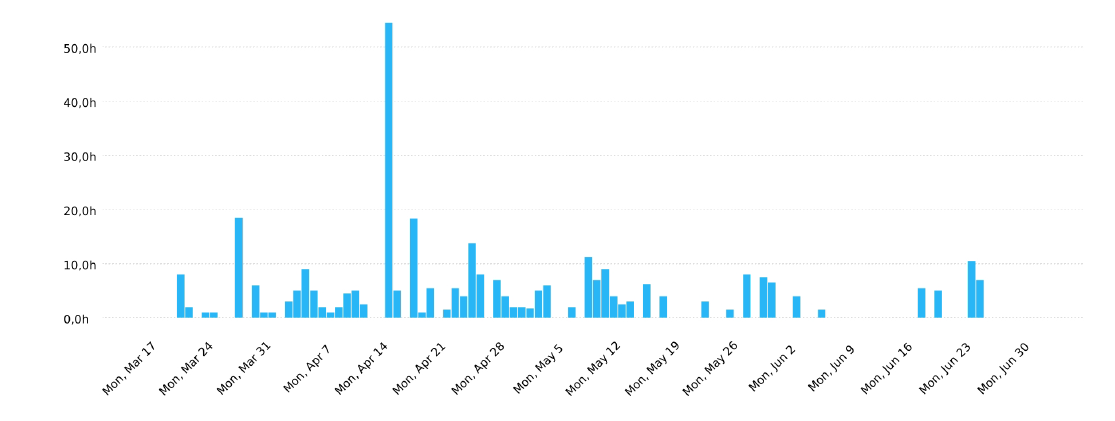
\includegraphics[width=\textwidth]{images/clockify_diagram.png}
    \caption{Gesamte Zeiterfassung mit Clockify}
    \label{fig:zeiterfassung}
\end{figure}

Die dargestellten Werte zeigen die insgesamt investierten Stunden, aufgeteilt nach Kalenderwochen. Die Daten umfassen die gesamte Projektlaufzeit und beziehen sich auf alle Teammitglieder gemeinsam. Die Stundenangaben sind jeweils in Stunden summiert.

Im Folgenden ist eine detaillierte Aufschlüsselung der investierten Zeit nach einzelnen Teammitgliedern zu sehen. Diese Darstellung vermittelt einen transparenten Überblick über die individuelle Arbeitsverteilung innerhalb des Teams sowie den Gesamtaufwand.

\begin{figure}[H]
    \centering
    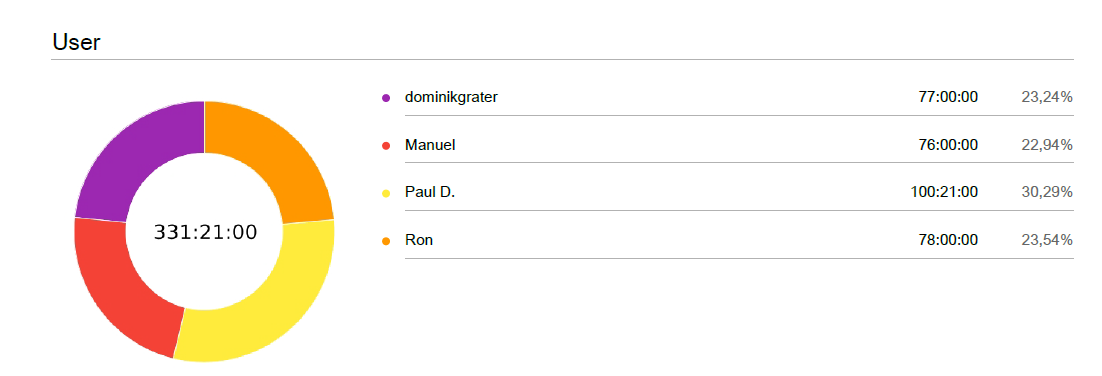
\includegraphics[width=\textwidth]{images/clockify_piechart.png}
    \caption{Aufteilung der Zeiterfassung nach Teammitgliedern}
    \label{fig:piechart}
\end{figure}
\newpage
\section{Fazit}
Die Entwicklung der Rocket App war ein anspruchsvolles, aber äußerst lehrreiches Projekt, das verschiedene Aspekte der modernen Softwareentwicklung praxisnah miteinander verknüpft hat.
Von der Planung über die Implementierung bis hin zum Deployment konnten wir nicht nur unser technisches Wissen vertiefen, sondern auch wichtige Erfahrungen in der Teamarbeit,
im Projektmanagement und in der interdisziplinären Kommunikation sammeln.
Besonders hervorzuheben ist die Vielschichtigkeit des Projekts: Die Kombination aus mobiler App, Backend-API, Webplattform und DevOps-Elementen wie Containerisierung und automatisiertem Deployment
stellte uns immer wieder vor neue Herausforderungen, die wir gemeinsam lösen konnten. Dabei haben sich Werkzeuge wie GitHub, Docker, Flutter und Go als wertvolle Technologien erwiesen.
Neben der technischen Umsetzung stand auch die Nutzererfahrung im Fokus: Durch Features wie Gamification, soziale Interaktion und eine ansprechende UI ist es uns gelungen, eine Anwendung zu schaffen,
die funktional und motivierend zugleich ist. Der Einsatz eines flexiblen Architekturdesigns und die Nutzung von Cloud-Infrastrukturen ermöglichen zudem eine langfristige Wartbarkeit und Erweiterbarkeit der App.
Abschließend lässt sich sagen, dass die Rocket App nicht nur ein erfolgreiches Ergebnis unseres Projektmoduls darstellt, sondern auch eine solide Basis für zukünftige Weiterentwicklungen bietet.
Das Projekt hat uns gezeigt, wie wichtig saubere Planung, strukturierte Umsetzung und kontinuierliches Feedback sind – Fähigkeiten, die wir auch in kommenden Projekten einsetzen werden.
\newpage
\section{Referenzen}

\begin{thebibliography}{9}
\bibitem{androidstudio}
Android Studio, \emph{Android Studio IDE}, \url{https://developer.android.com/studio}

\bibitem{docker}
Docker, \emph{Docker: Empowering App Development for Developers}, \url{https://www.docker.com/}

\bibitem{docker_hub}
Docker Hub zephiron, \emph{Docker Hub: Container Registry}, \url{https://hub.docker.com/u/zephiron}

\bibitem{flutter}
Flutter, \emph{Flutter - Beautiful native apps in record time}, \url{https://flutter.dev/}

\bibitem{flutter_foreground_task}
Flutter Foreground Task, \emph{Flutter Foreground Task Plugin}, \url{https://pub.dev/packages/flutter_foreground_task}

\bibitem{flutter_osm_plugin}
Flutter OSM Plugin, \emph{Flutter OSM Plugin for OpenStreetMap}, \url{https://pub.dev/packages/flutter_osm_plugin}

\bibitem{flutter_secure_storage}
Flutter Secure Storage, \emph{Flutter Secure Storage Plugin}, \url{https://pub.dev/packages/flutter_secure_storage}

\bibitem{ginkgo}
Ginkgo, \emph{Ginkgo: BDD Testing Framework for Go}, \url{https://onsi.github.io/ginkgo/}

\bibitem{github}
GitHub, \emph{GitHub: Where the world builds software}, \url{https://github.com/}

\bibitem{gomega}
Gomega, \emph{Gomega: Matcher Library for Go}, \url{https://onsi.github.io/gomega/}

\bibitem{golang}
Go, \emph{The Go Programming Language}, \url{https://golang.org/}

\bibitem{gopls}
Go Language Server Protocol, \emph{gopls: The Go Language Server}, \url{https://github.com/golang/tools/tree/master/gopls}

\bibitem{jwt}
JWT, \emph{JSON Web Tokens}, \url{https://jwt.io/}

\bibitem{migrate}
Migrate, \emph{Migrate: Database Migration Tool}, \url{https://github.com/golang-migrate/migrate}

\bibitem{nginx}
NGINX, \emph{NGINX Web Server}, \url{https://nginx.org/}

\bibitem{open_topo_data}
OpenTopoData, \emph{OpenTopoData: Open Topographic Data}, \url{https://opentopodata.org/}

\bibitem{openstreetmap}
OpenStreetMap, \emph{OpenStreetMap Project}, \url{https://www.openstreetmap.org/}

\bibitem{pedometer}
Pedometer, \emph{Flutter Pedometer Plugin}, \url{https://pub.dev/packages/pedometer}

\bibitem{postgresql}
PostgreSQL, \emph{The World's Most Advanced Open Source Relational Database}, \url{https://www.postgresql.org/}

\bibitem{testcontainers}
Testcontainers, \emph{Testcontainers for Go}, \url{https://golang.testcontainers.org/}

\bibitem{vite}
Vite, \emph{Vite: Next Generation Frontend Tooling}, \url{https://vitejs.dev/}

\bibitem{vuejs}
Vue.js, \emph{Vue.js: The Progressive JavaScript Framework}, \url{https://vuejs.org/}

\bibitem{VSCode}
Visual Studio Code, \emph{Visual Studio Code: Code Editing. Redefined}, \url{https://code.visualstudio.com/}

\bibitem{zed}
Zed, \emph{Zed: A modern code editor}, \url{https://zed.dev/}

\bibitem{everhour}
Everhour, \emph{Everhour: Time Tracking for Teams}, \url{https://everhour.com/}

\bibitem{clockify}
Clockify, \emph{Clockify: Free Time Tracking Software}, \url{https://clockify.me/}
\end{thebibliography}


\end{document}